\documentclass{article}

\usepackage{MGLassignment}

\newcommand\course{TΗΛ 311}
\newcommand\courseName{Στατιστική Μοντελοποίηση και Αναγνώριση Προτύπων}
\newcommand\semester{Χειμερινό 2020-2021}
\newcommand\assignmentNumber{1η Σειρά Ασκήσεων}
\newcommand\studentName{Μαυρογιώργης Δημήτρης}                           
\newcommand\studentNumber{2016030016}

\title{\underline{\textbf{\assignmentNumber}}} 
\author{\textsc{\textbf{Όνομα:}}  \studentName\\
		\textsc{\textbf{ΑΜ:}}  \studentNumber\\
		\course \ - \courseName\\ 
		\textsc{Πολυτεχνείο Κρήτης}
}
\date{\today}
\begin{document}
	\maketitle
\section*{Άσκηση 1: Principal Component Analysis (PCA)}
	Στο πρώτο μέρος της άσκησης κλήθήκαμε να υλοποιήσουμε τη μέθοδο PCA, για να μειώσουμε ις διαστάσεις των δεδομένων. Αρχικά, αφού διαβάστηκαν τα δεδομένα από το αρχείο 'ex1\_1\_data1.mat', έγινε μία κανονικοποίηση έτσι, ώστε να έχουν μέση τιμή 0 και συνδιασπορά 1. Για το λόγο αυτό συμπληρώθηκε ο κατάλληλος κώδικας στο αρχείο 'featureNormalize.m', όπου τα καινούρια δεδομένα υπολογίζονται με βάση τον τύπο $x_{new} = \frac{x_{old} - μ}{σ}$. Τα αποτελέσματα του normalization παρουσιάζονται παρακάτω.
	
	\begin{figure}[h!]
		\centering
		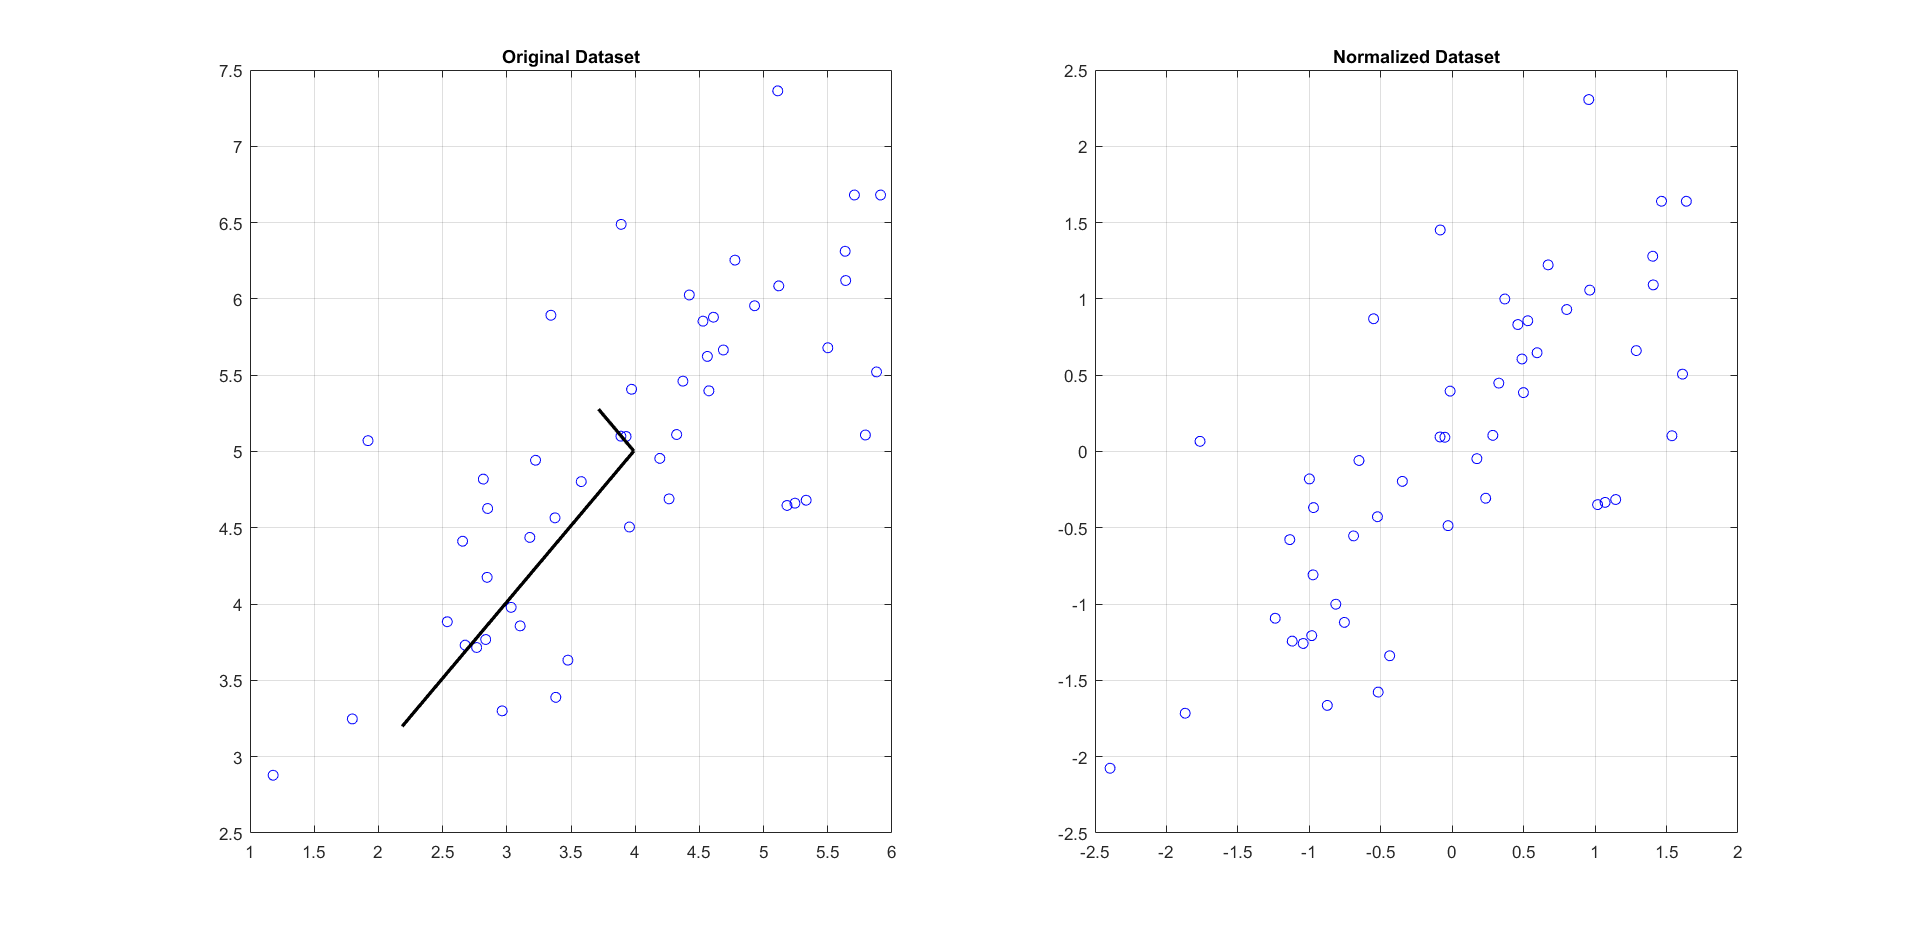
\includegraphics[width=\linewidth]{../exercise1_1/images/original_normalized_dataset.png}
	\end{figure}
	
	\noindent
	Στην συνέχεια, αφού γίνει η κανονικοποίηση των δεδομένων, πρέπει να υπολογίσουμε τις κύριες συνιστώσες του αλγορίθμου PCA (απεικονίζονται στο ίδιο subplot με τo original dataset). Έτσι, στο αρχείο 'myPCA.m' υπολογίζουμε τον πίνακα συνδιασποράς με βάση τον τύπο $\sum \frac{1}{m} X^{T}X$ όπου $X \in \Bbb R^{m \times n}$ είναι ένας πίνακας όπου κάθε γραμμή αντιστοιχεί σε ένα παράδειγμα με n χαρακτηριστικά. Tέλος, υπολογίζουμε τα ιδιοδιανύσματα και τις ιδιοτιμές του covariance matrix με τη χρήση της συνάρτησης svd() της Matlab.
	
	\noindent
	Κατόπιν, υπολογίζουμε την συνεισφορά που έχει κάθε κύρια συνιστώσα στην συνολική διακύμανση και
	έπειτα να εφαρμόζει τον αλγόριθμο PCA στα αρχικά δείγματα για να μειωθεί η διάστασή τους από 2D σε 1D. Γι' το λόγο αυτό στο αρχείο 'projectData.m' συμπληρώθηκε ο κατάλληλος κώδικας, με τον οποίο προβάλλουμε κάθε δείγμα $x_{i}$ στις Κ κύριες συνιστώσες με την εφαρμογή του
	γραμμικού μετασχηματισμού $z_{i} = U^{T}x_{i}$. 
	
	\noindent
	Μετά την προβολή των δεδομένων μπορούμε να ανακτήσουμε τα προσεγγιστικά δεδομένα επαναφέροντας τη διάστασή τους ξανά σε 2D. Έτσι, στο αρχείο 'recoverData.m' προβάλουμε τα δεδομένα πάνω σε όλες τις κύριες συνιστώσες σύμφωνα με το μετασχηματισμό  $x_{i,rec} = Uz_{i}$. Tα αποτελέσματα που προέκυψαν είναι τα εξής μετά από την παραπάνω διαδιακασία:
	
	\begin{figure}[h!]
		\centering
		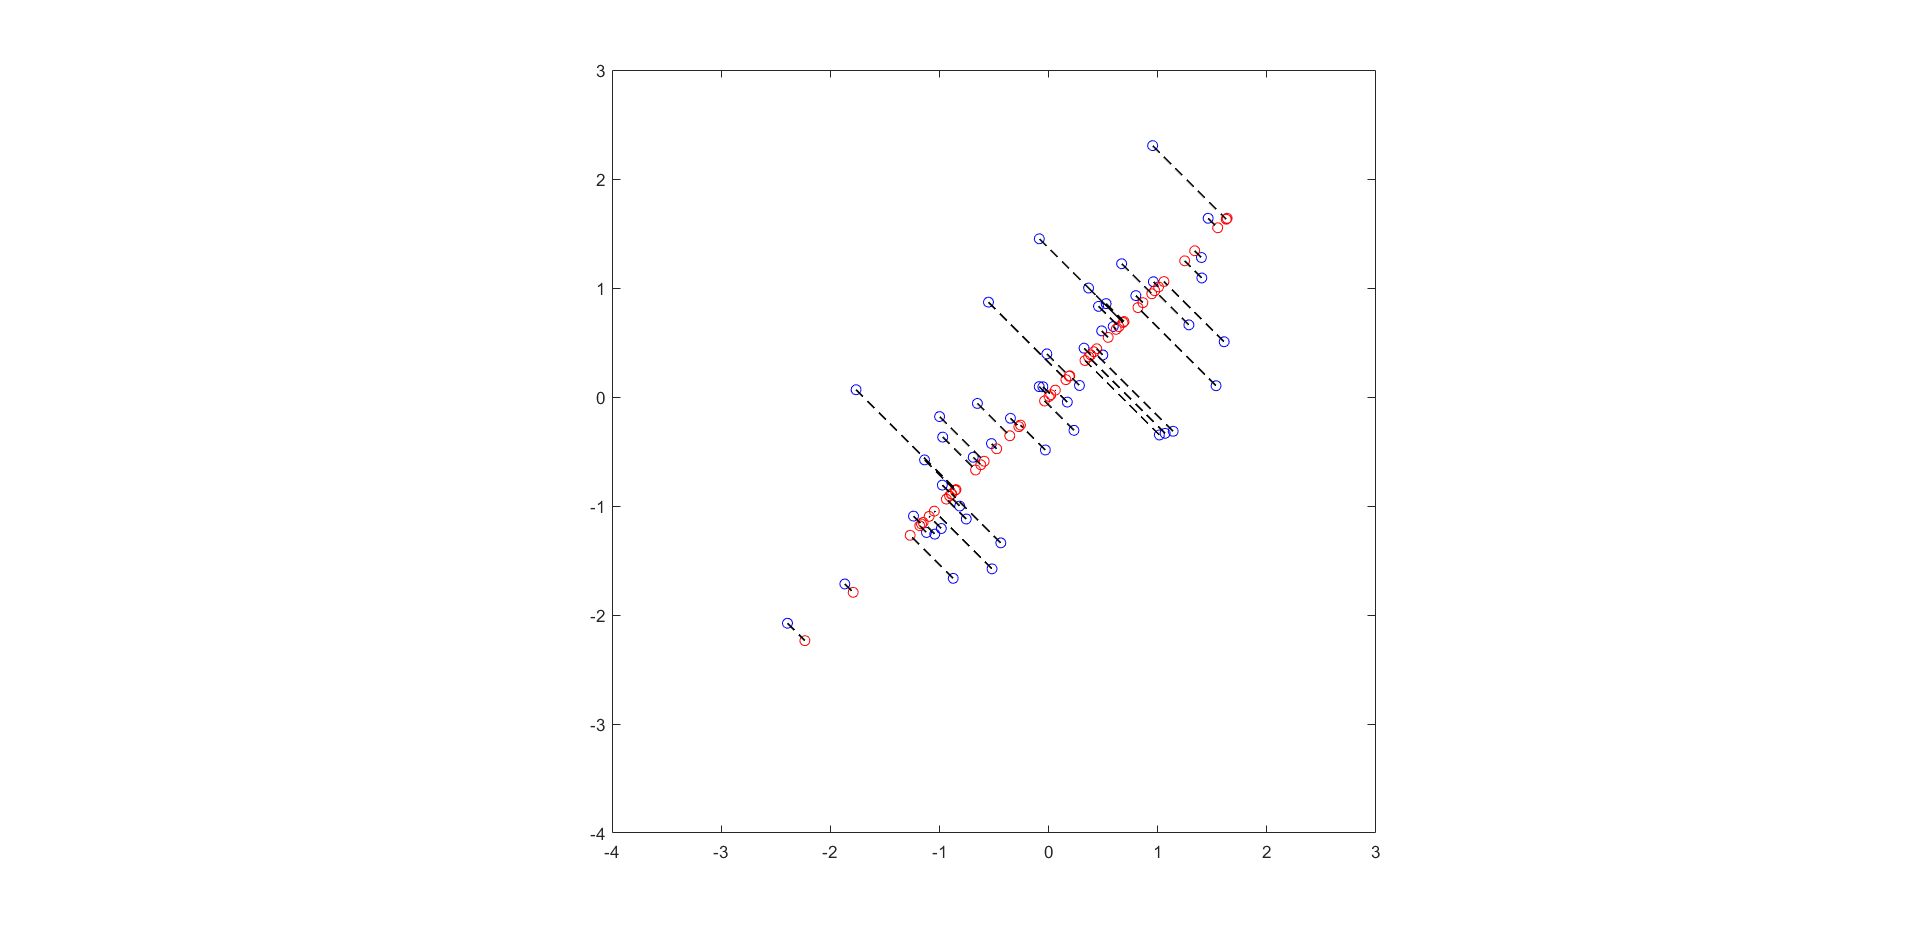
\includegraphics[width=\linewidth]{../exercise1_1/images/reconstructed_dataset.png}
	\end{figure}

	\noindent
	Στο δεύτερο μέρος της άσκησης κληθήκαμε να εφαρμόσουμε τη μέθοδο PCA σε ένα πραγματικό dataset από εικόνες διάφορων προσώπων. Αρχικά, αφού διαβάσουμε τις 100 πρώτες εικόνες και τις εμφανίσουμε με τη χρήση της συνάρτησης displayData() που η υλοποίησή της μας δίνεται έτοιμη, κάνουμε normalization των δειγμάτων, υπολογίζουμε τις κύριες συνιστώσες με τη συνάρτηση myPCA() και εμφανίζουμε τις 36 πρώτες κύριες συνιστώσες. Αυτό που παρατηρούμε είναι ότι απεικονίζονται τα 36 πρόσωπα των ιδιοδιανυσμάτων που υπολογίστηκαν από τη συνάρτηση myPCA().\\
	
	\noindent
	Κατόπιν, μειώνουμε τη διάσταση των δειγμάτων χρησιμοποιώντας τις 100 πρώτες συνιστώσες. Τέλος, εμφανίζουμε τα δείγματα μειωμένης διάστασης αφού πρώτα προβάλουμε στον αρχικό δειγματικό χώρο. Τα αποτελέσματα που προκύπτουν για Κ=100 είναι τα παρακάτω:
	
	 \begin{figure}[h!]
	 	\centering
	 	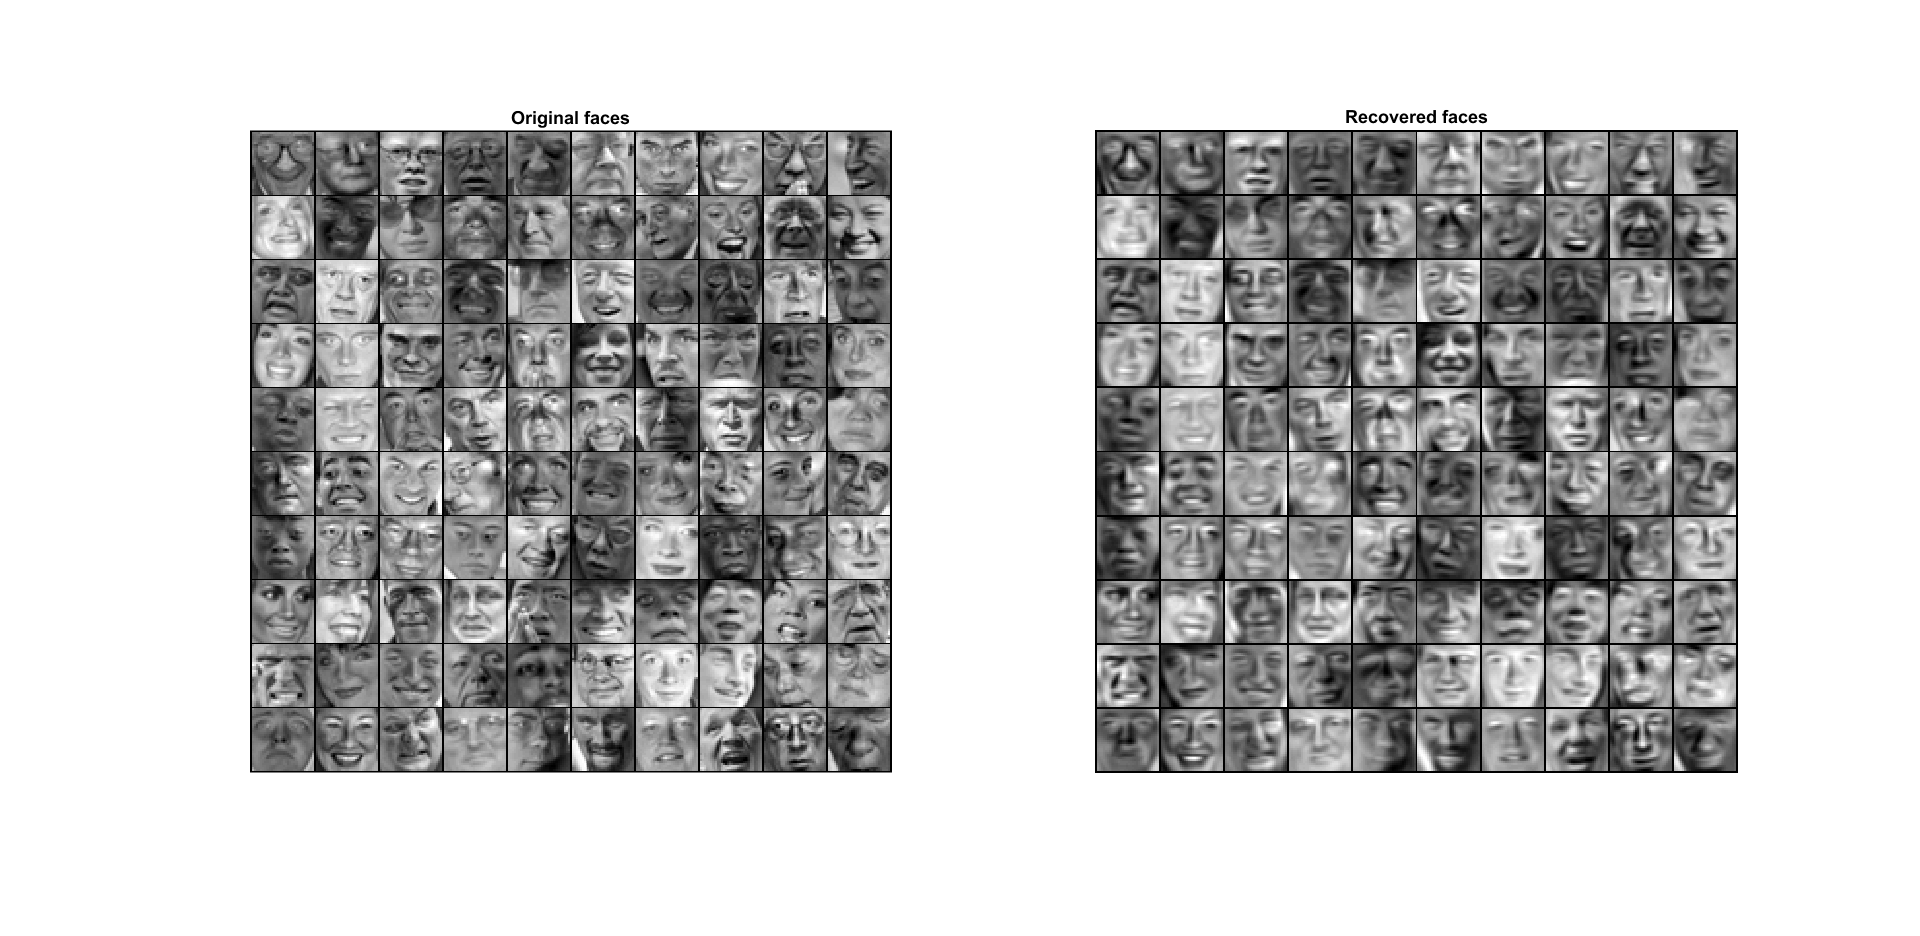
\includegraphics[height=6.5cm ,width=\linewidth]{../exercise1_1/images/faces_K_100.png}
	 	\caption{K=100 κύριες συνιστώσες}
	 \end{figure}
 
 	\noindent
 	Aυτό που παρατηρούμε είναι ότι οι ανακτημένες εικόνες είναι πιο θολες σε σχέση με τις αρχικές, δηλαδή υπάρχει κάποια μικρή απώλεια πληροφορίας. Tέλος, επαναλαμβάνουμε την παραπάνω διαδικασία για διάφορες τιμές των κύριων συνιστωσών. Παρακάτω βλέπουμε τις εικόνες που ανακτούμε για K=10, 50 και 200 κύριες συνιστώσες.
 	
 	\begin{figure}[h!]
 		\centering
 		\begin{subfigure}[t]{0.5\textwidth}
 			\centering
 			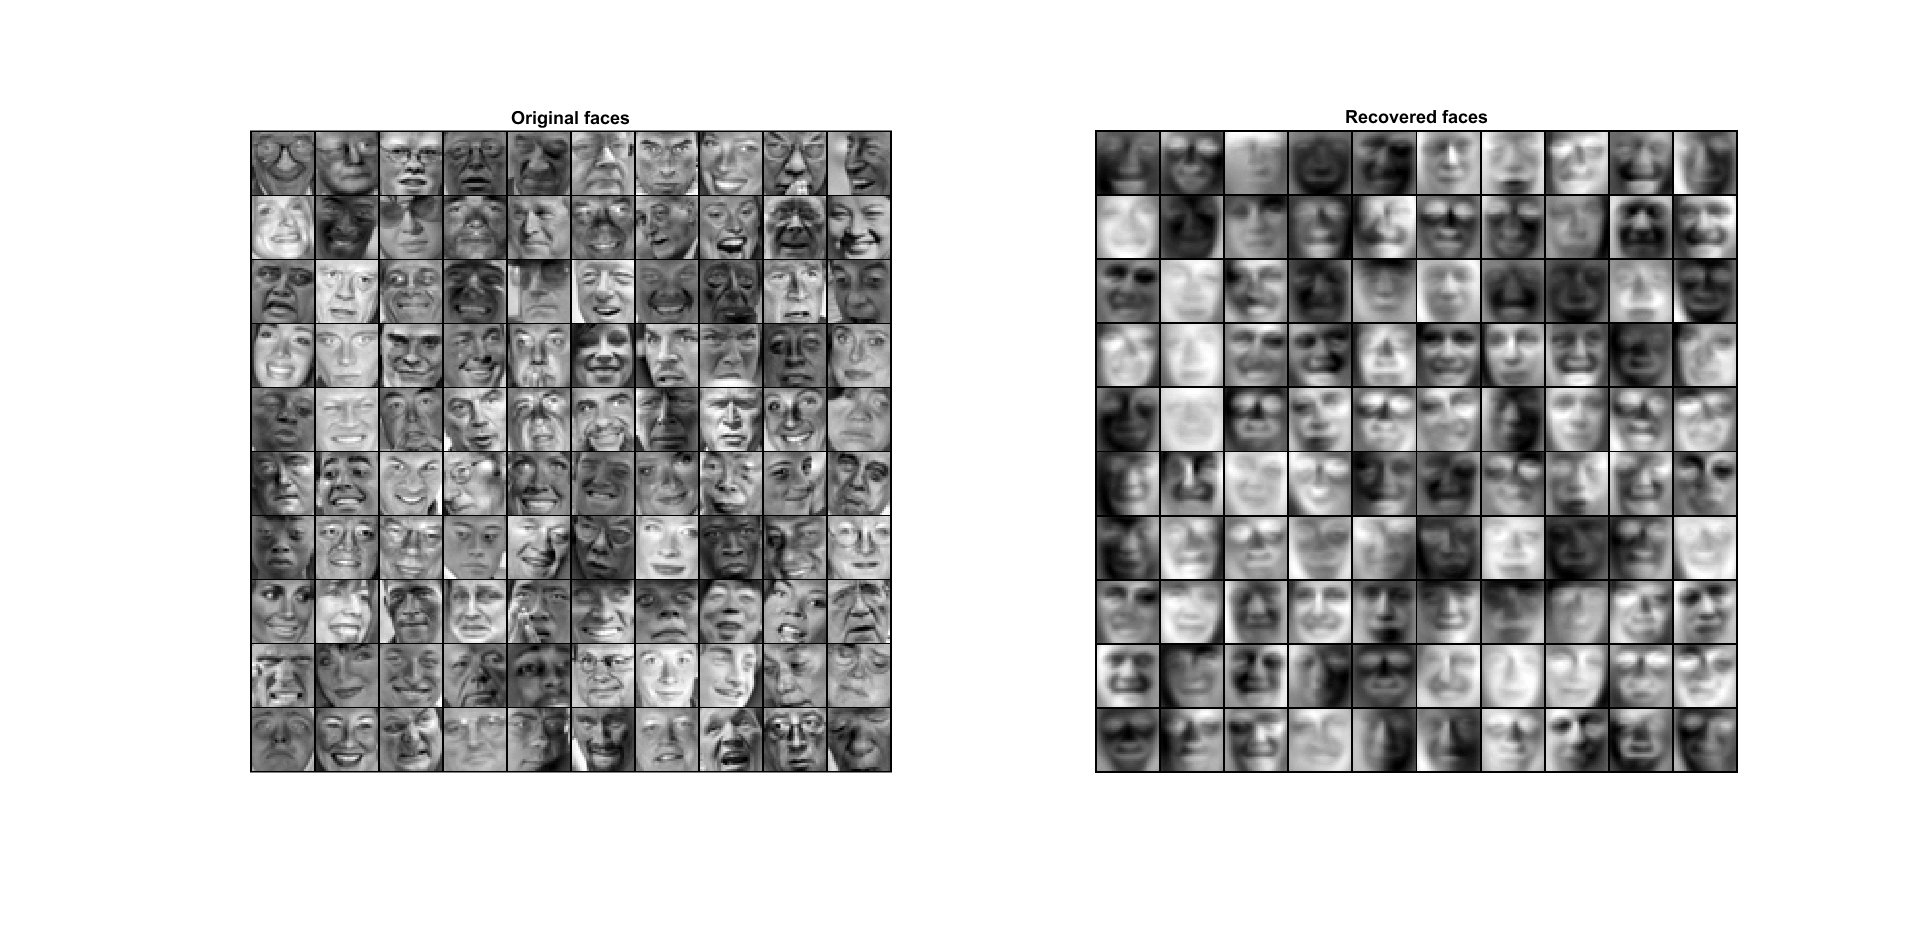
\includegraphics[height=5cm, width=\linewidth]{../exercise1_1/images/faces_K_10.png}
 			\caption{K=10 κύριες συνιστώσες}
 		\end{subfigure}%
 		~
 		\begin{subfigure}[t]{0.5\textwidth}
 			\centering
 			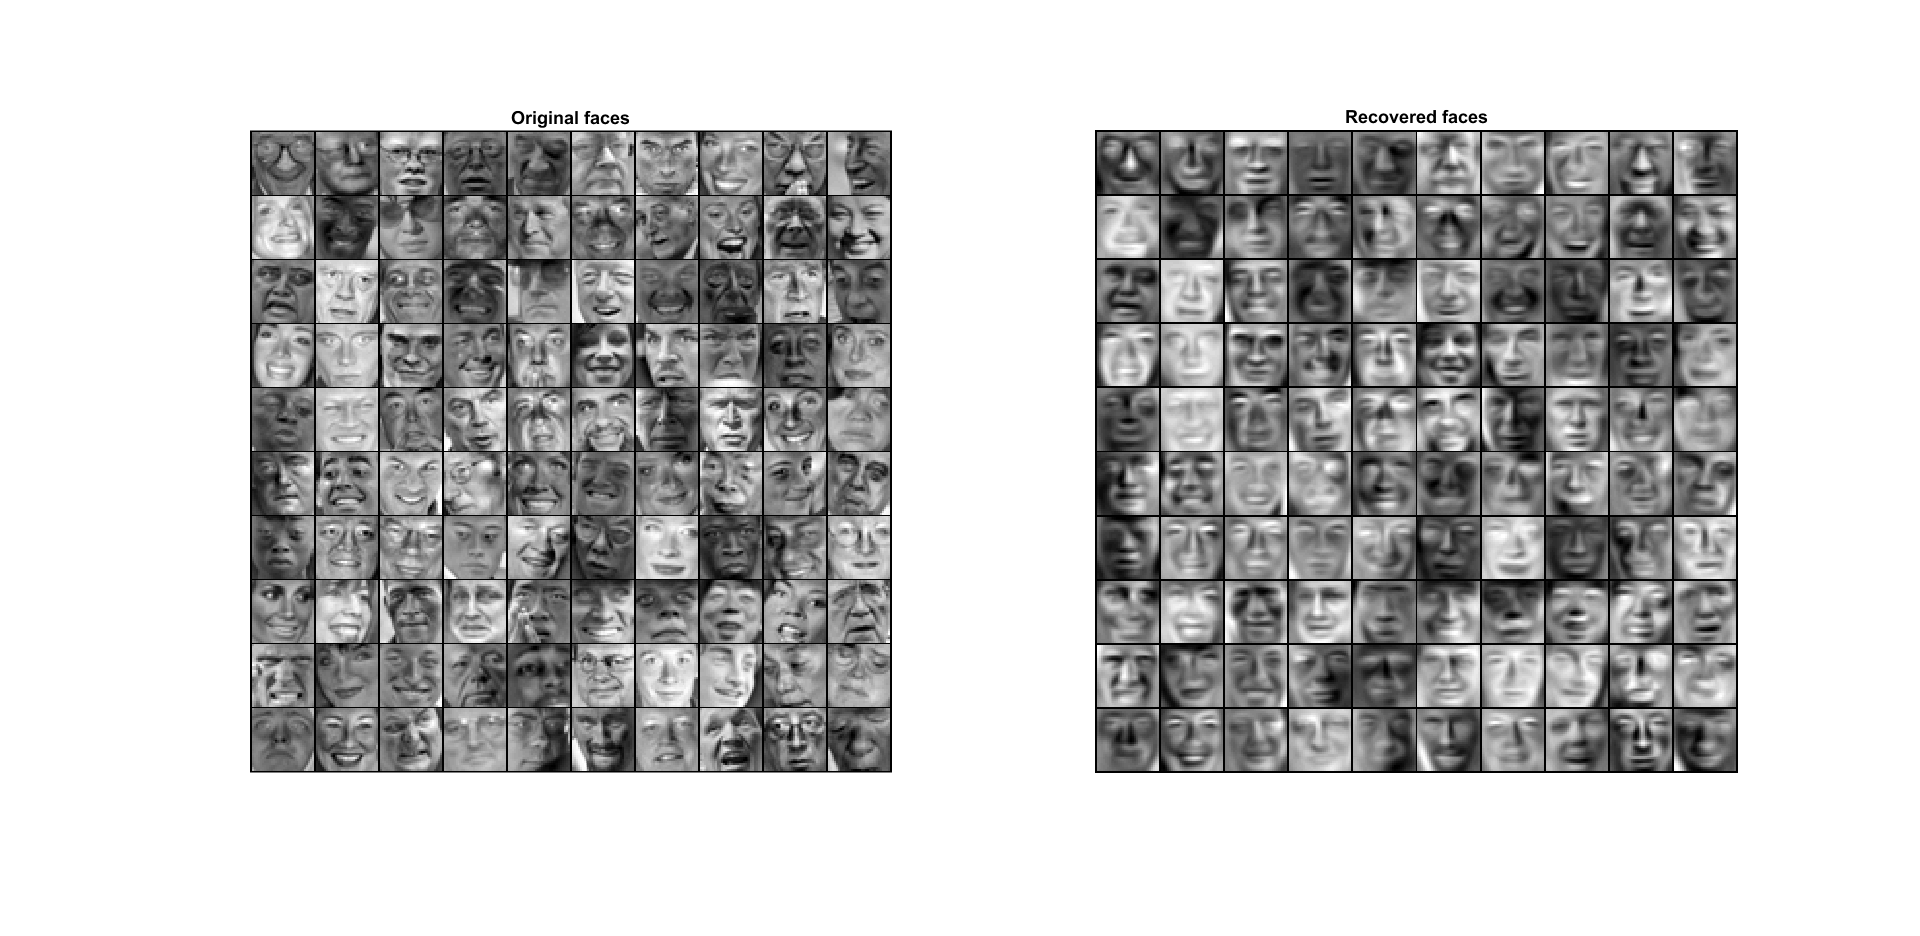
\includegraphics[height=5cm, width=\linewidth]{../exercise1_1/images/faces_K_50.png}
 			\caption{K=50 κύριες συνιστώσες}
 		\end{subfigure}
 	
 		\begin{subfigure}[t]{0.5\textwidth}
 			\centering
 			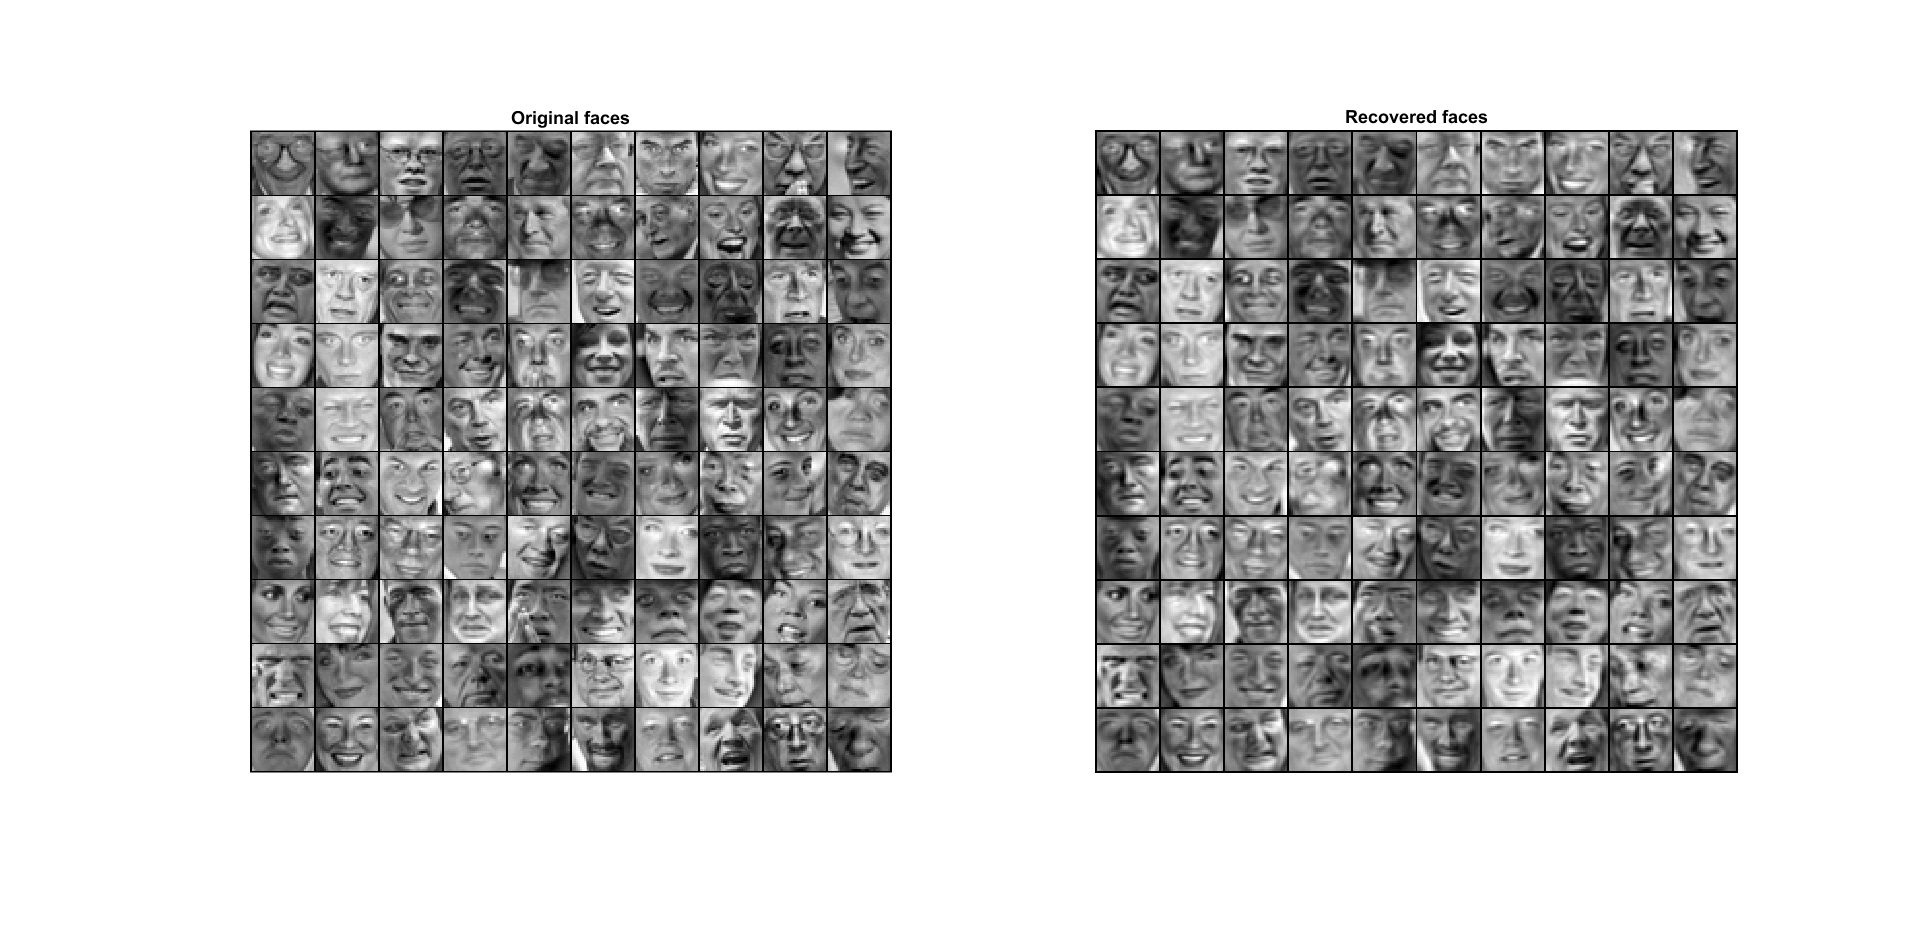
\includegraphics[height=5cm, width=\linewidth]{../exercise1_1/images/faces_K_200.png}
 			\caption{K=200 κύριες συνιστώσες}
 		\end{subfigure}
 	\end{figure}
 	
 	\noindent
 	Στην περίπτωση που δικιμάσουμε για K=10, 50 και 200 παρατηρούμε ότι όσο μειώνονται οι κύριες συνιστωσες οι εικόνες που ανακτούμε γίνονται ακόμη πιο θολές. Αντίθετα, αν αυξήσουμε τις κύριες συνιστώσες βλέπουμε ότι βελτιώνονται τα αποτελέσματα, δηλαδή έχουμε λιγότερη απώλεια πληροφορίας στις εικόνες των προσώπων.
 	
\section*{Άσκηση 2: Σχεδιάστε ένα ταξινομητή LDA (Linear Discriminant Analysis)}
	Έστω δύο ισοπίθανες κλάσεις $ω_1$, $ω_2$ , οι κατανομές των οποίων είναι Γκαουσιανές. Οι πίνακες συνδιασποράς και οι μέσες τιμές έχουν εκτιμηθεί ως εξής: 
	\begin{align*}
		μ_{1} = \begin{bmatrix}
					-5 \\
					5
				\end{bmatrix}	
		\tab
		μ_{2} = \begin{bmatrix}
					10 \\
					15
				\end{bmatrix}	\\	
		Σ_{1} = \begin{bmatrix}
			11 & 9 \\
			9 & 11
		\end{bmatrix}	
		\tab
		Σ_{2} = \begin{bmatrix}
			2 & 0 \\
			0 & 2
		\end{bmatrix}\\
	\end{align*}
	
	\pagebreak
	\noindent
	Το διάνυσμα προβολής w υπολογίζεται με βάση τον τύπο
	\begin{align*}
		w &= S_{w}^{-1} \cdot (μ_{1} - μ_{2}), \ \ \ 
		\text{όπου} \  \  \ 
		S_{w} = \frac{1}{2} \sum_{i=1}^{n} Σ_{i}\\ \\
		S_{w} &= \frac{1}{2} 
				 \begin{bmatrix}
				 	 11 & 9 \\
					 9 & 11
				 \end{bmatrix} + 
				 \frac{1}{2} 
				 \begin{bmatrix}
					 2 & 0 \\
					 0 & 2
				 \end{bmatrix}
			  = \frac{1}{2} 
				 \begin{bmatrix}
				 	13 & 9 \\
				  	9 & 13
				 \end{bmatrix}
			 = \begin{bmatrix}
				 	13/2 & 9/2 \\
				 	9/2 & 13/2
			   \end{bmatrix}\\ \\
		S_{w}^{-1} &= \frac{1}{\frac{13}{2}\frac{13}{2} - \frac{9}{2}\frac{9}{2}} 
					  \begin{bmatrix}
					  	13/2 & -9/2 \\
					  	-9/2 & 13/2
					  \end{bmatrix} = 
				  =  \frac{1}{22}
					 \begin{bmatrix}
					 	13/2 & -9/2 \\
					  	-9/2 & 13/2
					 \end{bmatrix}
				 = 	\begin{bmatrix}
					 	13/44 & -9/44 \\
					 	-9/44 & 13/44
					\end{bmatrix}\\ \\
		μ &= μ_{1} - μ_{2} = \begin{bmatrix}
								-5 \\
								5 
							\end{bmatrix} - 
							\begin{bmatrix}
								10 \\
								15
							\end{bmatrix}
						  = \begin{bmatrix}
								10 \\
								15
						  	\end{bmatrix}
					  	  = \begin{bmatrix}
						  	  	-13 \\
						  	  	-10
						  	\end{bmatrix}
	\end{align*}

	\noindent
	Συνεπώς, καταλήγουμε στο διάνυσμα προβολής
	\begin{align*}
		w &= S_{w}^{-1} \cdot μ
		   = \begin{bmatrix}
			   	13/44 & -9/44 \\
			   	-9/44 & 13/44
		     \end{bmatrix} \cdot
	     	 \begin{bmatrix}
	     	 	-13 \\
	     	 	-10
	     	 \end{bmatrix}
     	   = \begin{bmatrix}
	     	   	(-13 \cdot 13 + 9 \cdot 10)/44 \\
	     	   	(9 \cdot 15 - 13 \cdot 10)/44
     	   	 \end{bmatrix}	  
           = \begin{bmatrix}
	           	-105/44 \\
	           	5/44
             \end{bmatrix}   	
	\end{align*}
	
\section*{Άσκηση 3: Linear Discriminant Analysis (LDA) vs PCA}
	Ο σκοπός του πρώτου μέρους της άσκησης είναι εφαρμόσουμε Linear Discriminant Analysis έτσι, ώστε να μειώσουμε τη διάσταση ενός feature vector και να συγκρίνουμε τα αποτελέσματα αυτά με τη μέθοδο PCA. 
	
	\noindent
	Aρχικά, διαβάζουμε τα δεδομένα και εφαρμόζουμε μία κανονικοποίηση με μέση τιμή 0 και διασπορά 1. Για το normalization χρησιμοποιήθηκε η συνάρτηση featureNormalize όπως έγινε και στην άσκηση 1. \\
	
	\noindent
	Στη συνέχεια, για την υλοποίηση του fisherLinearDiscriminant υπολογίζουμε τις μέσες τιμές και τις διασπορές των δύο κλάσεων και στη συνέχεια με βάση τους τύπους που χρησιμοποιήθηκαν στην άσκηση 2 υπολογίζουμε το within class $S_{w}$, το διάνυσμα προβολής w και το κανονικοποιημένο διάνυσμα προβολής w.\\
	
	\noindent
	Για να μειώσουμε τη διάσταση των δεδομένων σε 1D προστέθηκε ο κατάλληλος κώδικας στο αρχείο 'projectLDA.m' όπου στο συγκεκριμένο απλώς υπολογίζουμε τον πίνακα δεδομένων $Z = X \cdot v$. Τέλος, στο αρχείο 'recoverLDA.m' κάνουμε ανακατασκευή των δειγμάτων μειωμένης διάστασης στον δισδιάστατο χώρο προβάλλοντας τα πάνω στην κατεύθυνση του διανύσματος προβολής LDA. Οπότε προκύπτουν τα recover δείγματα με βάση τον τύπο $x_{rec} = Z \cdot v^{T}$. Στα ίδια δείγματα εφαρμόστηκε ο αλγόριθμος PCA που υλοποιήθηκε στην άσκηση 1 οπότε έχουμε τα εξής αποτελέσματα έπειτα από την εφαρμογή του, καθώς και τα αποτελέσματα του αλγορίθμου LDA φαίνονται παρακάτω
	
	\pagebreak
 	\begin{figure}[h!]
		\centering
		\begin{subfigure}[t]{0.5\textwidth}
			\centering
			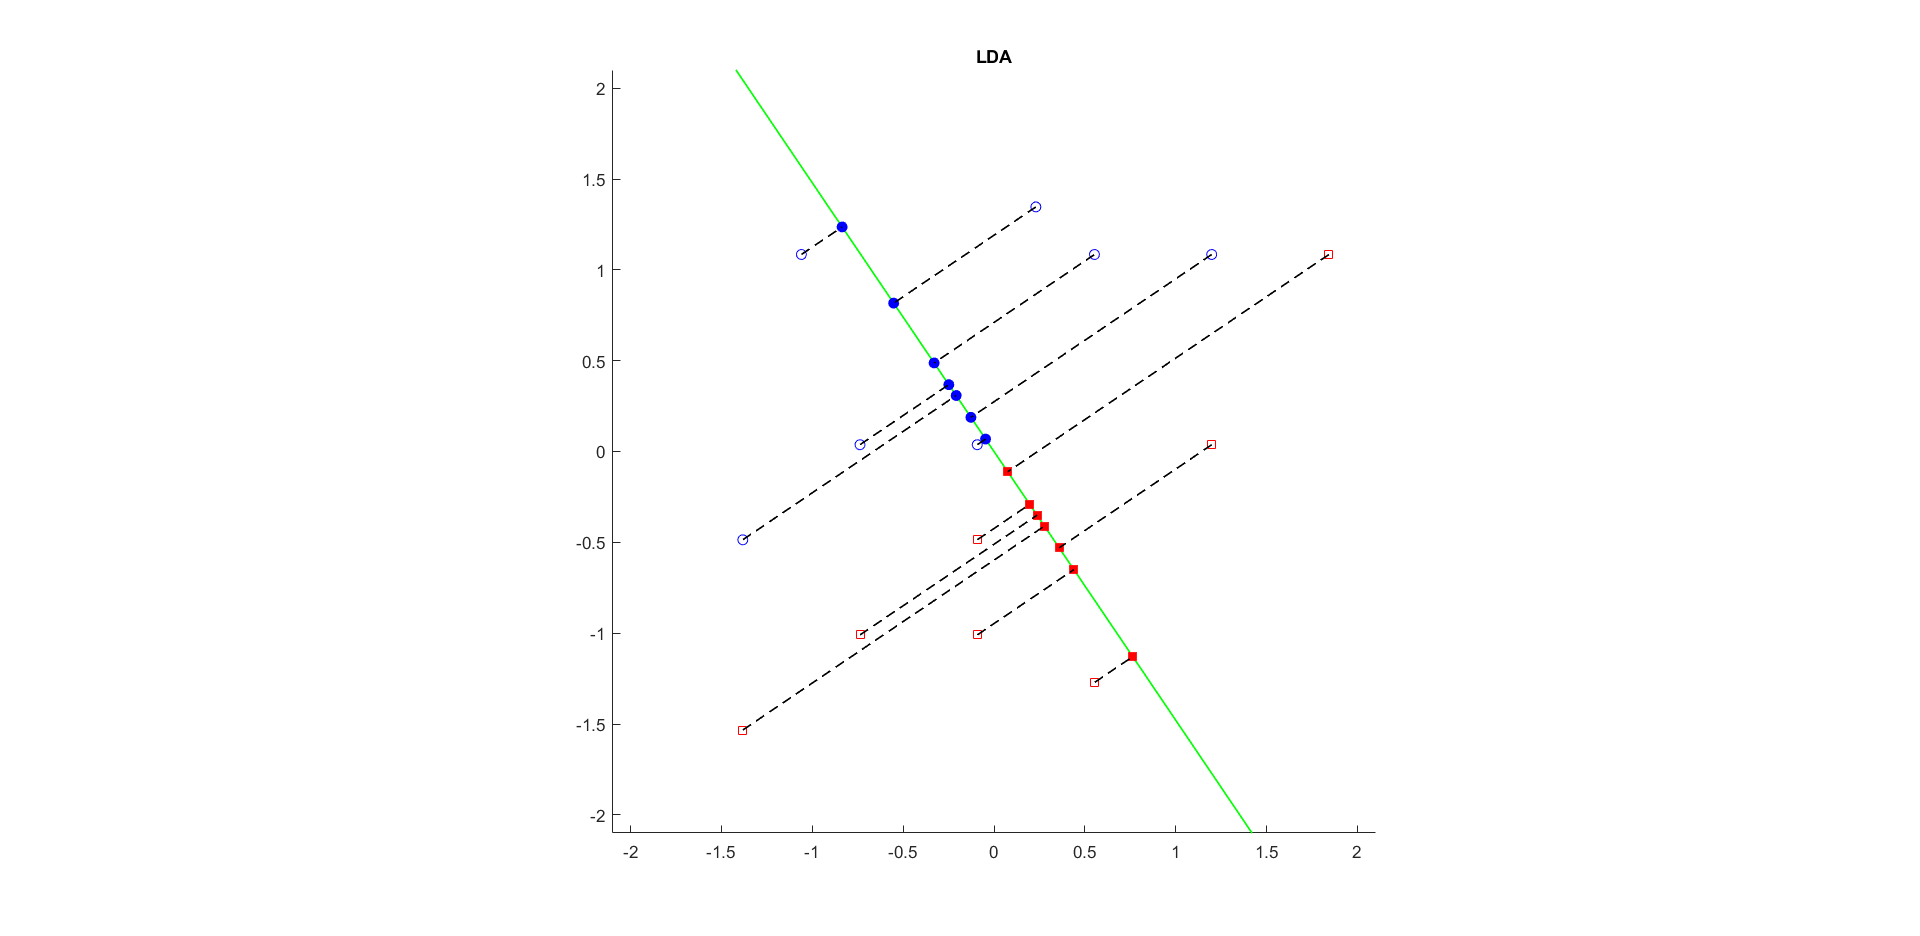
\includegraphics[width=\linewidth]{../exercise1_3/images/lda.png}
			\caption{LDA algorithm}
		\end{subfigure}%
		~
		\begin{subfigure}[t]{0.5\textwidth}
			\centering
			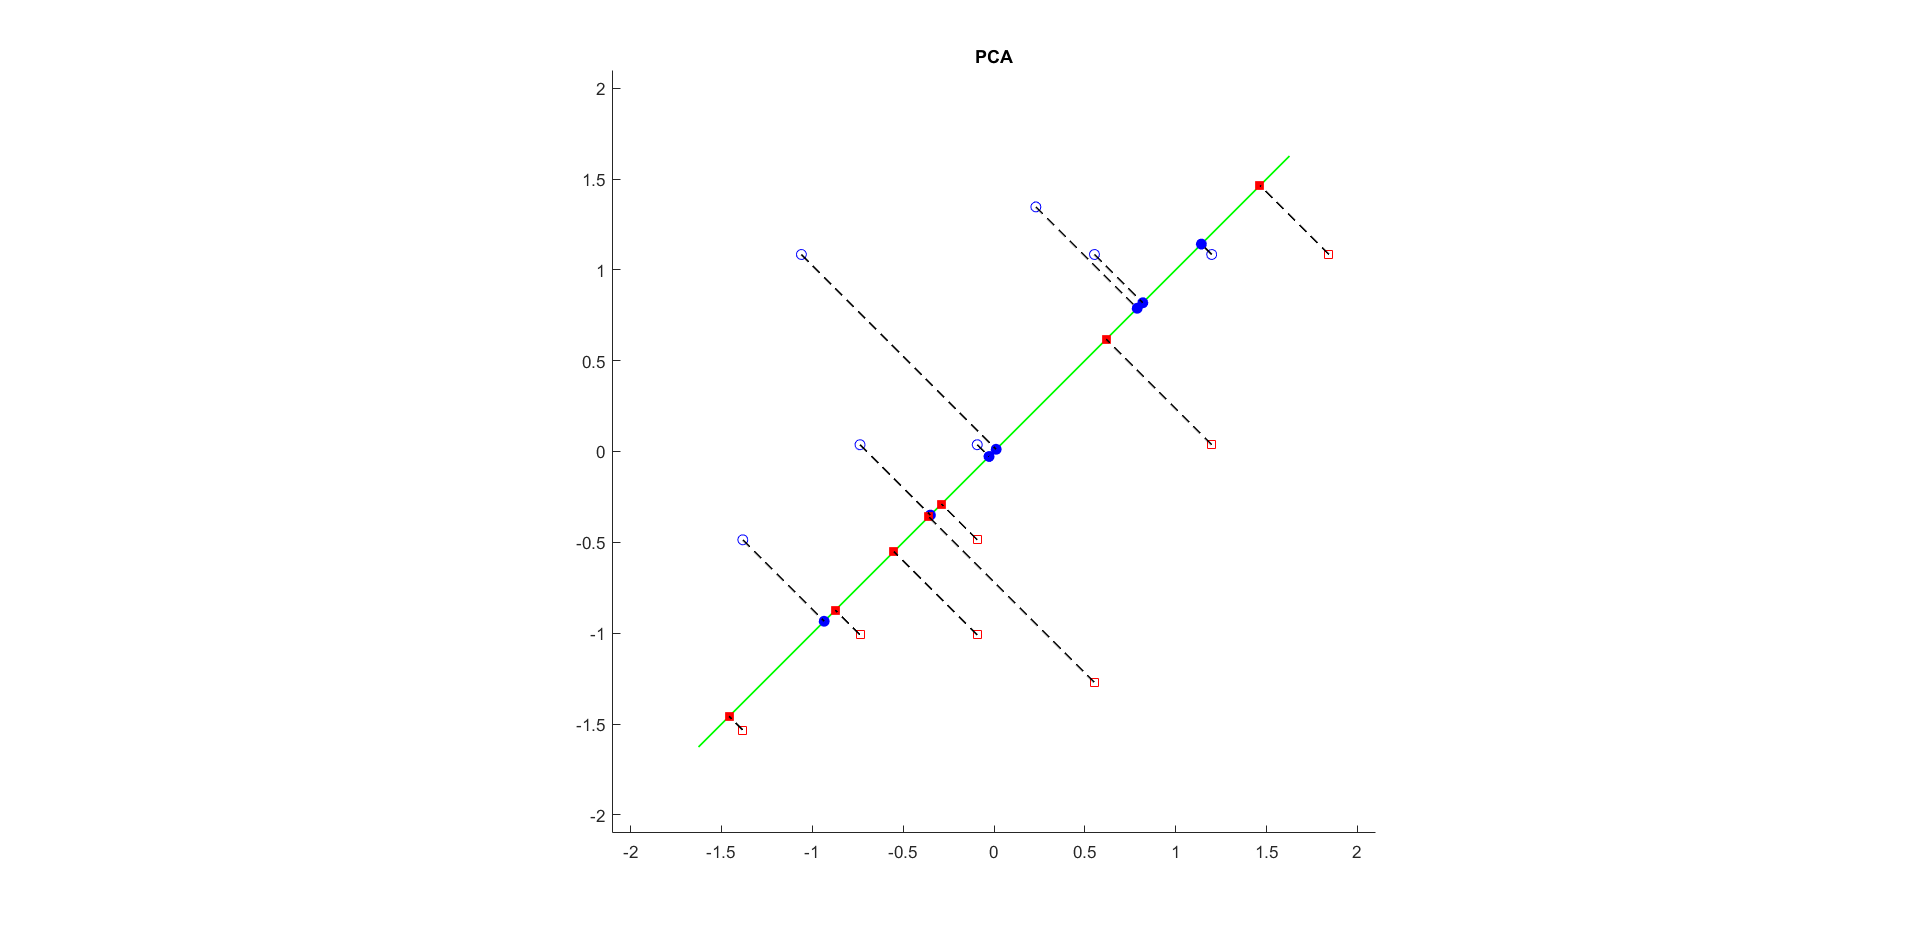
\includegraphics[width=\linewidth]{../exercise1_3/images/pca.png}
			\caption{PCA algorithm}
		\end{subfigure}
	\end{figure}

	\noindent
	Aυτό που παρατηρούμε από τα παραπάνω αποτελέσματα των δύο αργορίθμων είναι ότι ο αλγόριθμος LDA διαχωρίζει καλύτερα τα δεδομένα σε 2 κλάσεις χωρίς να υπάρχει επικάλυψη της μίας κλάσης με την άλλη. Aντίθετα, βλέπουμε ότι στον αλγόριθμο PCA, τα δείγματα της μίας κλάσης επικαλύπτονται με της άλλης και, επομένως, δεν υπάρχει ξεκάθαρος διαχωρισμός των δειγμάτων σε δύο διαφορετικές κλάσεις.\\ 
	
	\noindent
	Στο δεύτερο μέρος της άσκησης εφαρμόζουμε τον αλγόριθμο LDA στη βάση
	δεδομένων Iris, η οποία περιέχει δείγματα από 3 διαφορετικά είδη της οικογεένειας λουλουδιών Iris.\\
	
	\noindent
	Όπως και στο πρώτο μέρος εφαρμόστηκε πριν τον αλγόριθμο μια κανονικοποίηση των δειγμάτων. Στη συνέχεια, στη συνάρτηση myLDA() υπολογίζουμε τις prior πιθανότητες κάθε κλάσης, τις μέσες τιμές, τον ολικό μέσο, τους πίνακες within-class και between-class και τον πίνακα $S_{w}^{-1}\cdot S_{b}$ του γενικευμένου συστήματος ιδιοτιμών, στον οποίο εφαρμόζετε eigendecomposition. Tέλος, εφαρμόζουμε τα διανύσματα προβολής πάνω στα αρχικά δείγματα με τη συνάρτηση projectDataLDA έτσι ώστε να μειώσουμε τη διάσταση του σε 2D. Τα αποτελέσματα που προέκυψαν είναι τα εξής:
	
	 \begin{figure}[h!]
		\centering
		\begin{subfigure}[t]{0.5\textwidth}
			\centering
			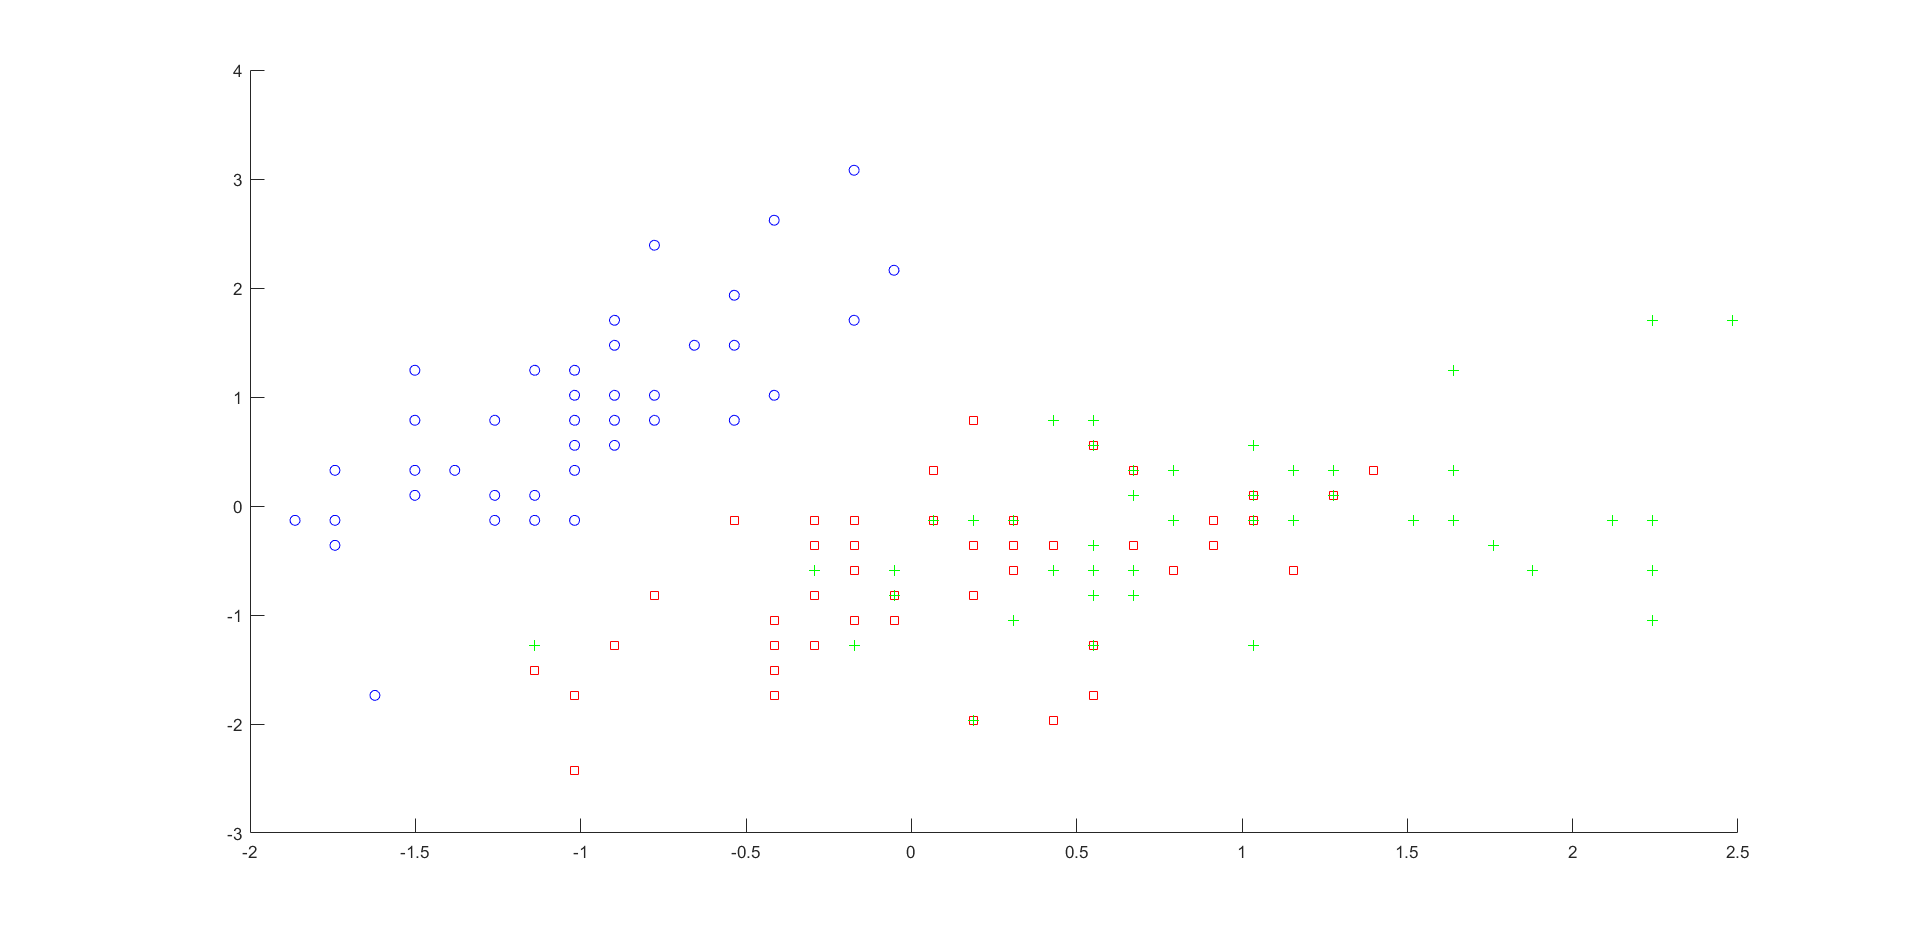
\includegraphics[width=\linewidth]{../exercise1_3/images/flowers_dataset.png}
			\caption{Dataset}
		\end{subfigure}%
		~
		\begin{subfigure}[t]{0.5\textwidth}
			\centering
			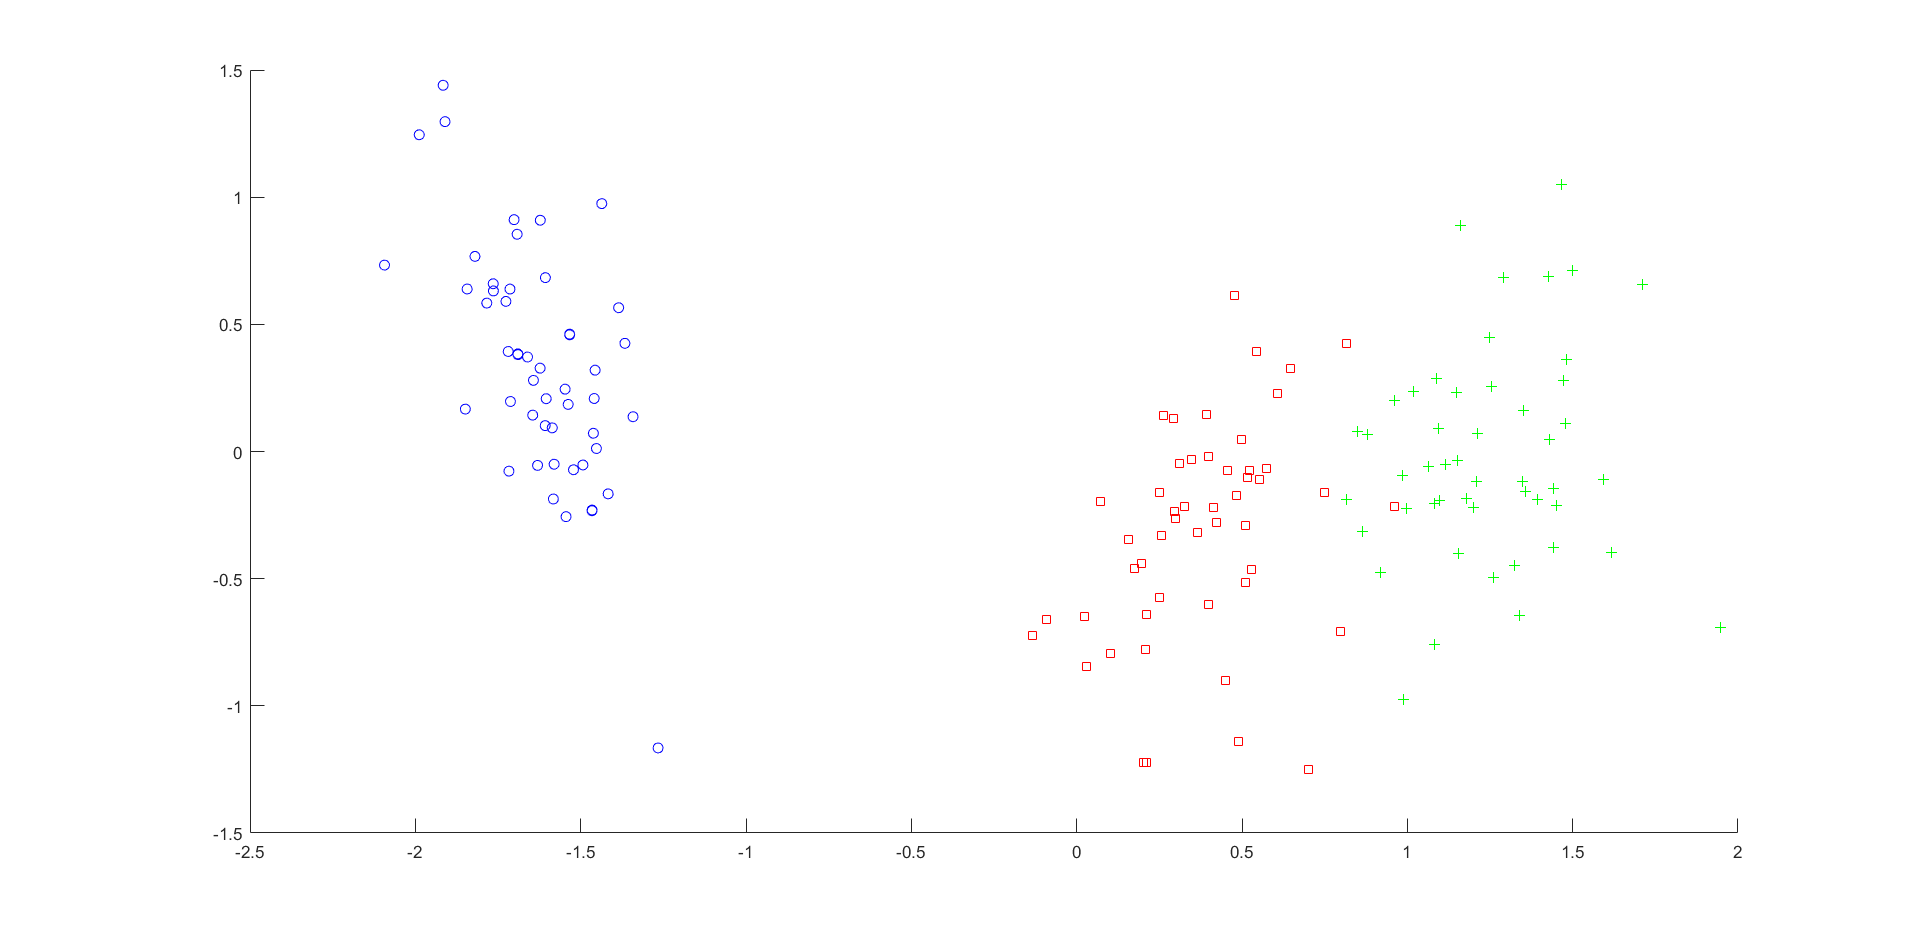
\includegraphics[width=\linewidth]{../exercise1_3/images/flowers_lda.png}
			\caption{LDA algorithm}
		\end{subfigure}
	\end{figure}

	\noindent
	Aυτό που προκύπτει ως συμπέρασμα από την εφαρμογή του αλγορίθμου LDA στο dataset είναι ότι υπάρχει διαχωρισμός των δειγμάτων σε 3 διαφορετικές κλάσεις. Ωστόσο, μεταξύ της κόκκινης κλάσης και της πράσινης δεν υπάρχει πλήρης διαχωρισμός, καθώς βλέπουμε ότι κάποια ελάχιστα δείγματα της κόκκινης κλάσης εμπεριέχονται ή είναι αρκετά κοντά στην πράσινη κλάση.

\pagebreak
\section*{Άσκηση 4: Bayes}	
	Έστω δύο κλάσεις $ω_{1}$ και $ω_{2}$ των οποίων οι εκ των προτέρων
	πιθανότητες είναι P($ω_{1}$) και P($ω_{2}$) αντίστοιχα. Τα δείγματα x που πρέπει να κατηγοριοποιηθούν είναι δισδιάστατα και οι κλάσεις περιγράφονται από τις ακόλουθες κανονικές κατανομές: 
	
	\begin{align*}
		P(x | ω_{1}) = N(μ_{1}, Σ_{1}), \tab P(x | ω_{2}) = N(μ_{2}, Σ_{2})\\\\
		μ_{1} = \begin{bmatrix}
			3 \\
			3
		\end{bmatrix}	
		\tab
		μ_{2} = \begin{bmatrix}
			6 \\
			6
		\end{bmatrix}	\\	
		Σ_{1} = \begin{bmatrix}
			1.2 & -0.4 \\
			-0.4 & 1.2
		\end{bmatrix}	
		\tab
		Σ_{2} = \begin{bmatrix}
			1.2 & 0.4 \\
			0.4 & 1.2
		\end{bmatrix}\\
	\end{align*}

	\noindent
	Με βάση τον κανόνα απόφασης έχουμε τα εξής:
	\begin{itemize}
		\item x = $ω_{1}$ αν P($ω_{1}$ | x) > P( $ω_{2}$ | x)
		\item x = $ω_{2}$ αν P($ω_{1}$ | x) < P( $ω_{2}$ | x)
	\end{itemize}
	
	\noindent
	Για να βρούμε το όριο απόφασης, αρκέι να λύσουμε την παρακάτω εξίσωση
	
	\begin{align*}
		P(ω_{1} | x) &= P( ω_{2} | x) \Rightarrow \\
		\frac{P(x | ω_{1}) \cdot P(ω_{1})}{P(x)} &= \frac{P(x | ω_{2}) \cdot P(ω_{2})}{P(x)} \Rightarrow \\
		P(x | ω_{1}) \cdot P(ω_{1}) &= P(x | ω_{2}) \cdot P(ω_{2}) \\
	\end{align*}

	\noindent
	Eπιπλέον, γνωρίζουμε ότι 
	\begin{align*}
		P(x | ω_{i}) = \frac{1}{\sqrt{2π} |Σ_{i}|} e^{-\frac{1}{2}(x - μ_{i})^{T} Σ_{i}^{-1} (x - μ_{i})}
	\end{align*}
	
	\noindent
	Όσον αφορά τις ορίζουσες των πινάκων συνδιασποράς έχουμε ότι \\
	$|Σ_{1}| = 1.2^2 - (-0.4)^2 = 1.28$ \ \ και \ \ $|Σ_{2}| = 1.2^2 - 0.4^2 = 1.28$\\
	
	\begin{align*}
		P(x | ω_{1}) \cdot P(ω_{1}) &= P(x | ω_{2}) \cdot P(ω_{2}) \\
		\frac{1}{\sqrt{2π} |Σ_{1}|} e^{-\frac{1}{2}(x - μ_{1})^{T} Σ_{1}^{-1} (x - μ_{1})} \cdot P(ω_{1}) &= 
		\frac{1}{\sqrt{2π} |Σ_{2}|} e^{-\frac{1}{2}(x - μ_{2})^{T} Σ_{i}^{-1} (x - μ_{2})} \cdot P(ω_{2}) \\
		e^{-\frac{1}{2}(x - μ_{1})^{T} Σ_{1}^{-1} (x - μ_{1})} \cdot P(ω_{1}) &= 
		e^{-\frac{1}{2}(x - μ_{2})^{T} Σ_{i}^{-1} (x - μ_{2})} \cdot P(ω_{2}) \\
		-\frac{1}{2}(x - μ_{1})^{T} Σ_{1}^{-1} (x - μ_{1}) + \ln (P(ω_{1})) &= 
		-\frac{1}{2}(x - μ_{2})^{T} Σ_{i}^{-1} (x - μ_{2}) + \ln (P(ω_{2})) 
	\end{align*}

	\begin{align*}
		\ln \left(\frac{P(ω_{1})}{P(ω_{2})}\right) = 
		\frac{1}{2}
		\begin{bmatrix}
			x_{1} - 3 &	x_{2} - 3
		\end{bmatrix} 
		\frac{1}{1.28}
		\begin{bmatrix}
			1.2 & 0.4 \\
			0.4 & 1.2
		\end{bmatrix}
		\begin{bmatrix}
			x_{1} - 3 \\
			x_{2} - 3
		\end{bmatrix} - 
		\frac{1}{2}
		\begin{bmatrix}
			x_{1} - 6 &	x_{2} - 6
		\end{bmatrix} 
		\frac{1}{1.28}
		\begin{bmatrix}
			1.2 & -0.4 \\
			-0.4 & 1.2
		\end{bmatrix}
		\begin{bmatrix}
			x_{1} - 6 \\
			x_{2} - 6
		\end{bmatrix} \\
		\ln \left(\frac{P(ω_{1})}{P(ω_{2})}\right) = 
		\begin{bmatrix}
			x_{1} - 3 &	x_{2} - 3
		\end{bmatrix} 
		\begin{bmatrix}
			0.46875 & 0.15625 \\
			0.15625 & 0.46875
		\end{bmatrix}
		\begin{bmatrix}
			x_{1} - 3 \\
			x_{2} - 3
		\end{bmatrix} - 
		\begin{bmatrix}
			x_{1} - 6 &	x_{2} - 6
		\end{bmatrix} 
		\begin{bmatrix}
			0.46875 & -0.15625 \\
			-0.15625 & 0.46875
		\end{bmatrix}
		\begin{bmatrix}
			x_{1} - 6 \\
			x_{2} - 6
		\end{bmatrix} \\
	\end{align*}
	
	\begin{align*}
		\ln \left(\frac{P(ω_{1})}{P(ω_{2})}\right) = 
		(x1 - 3) \cdot ( 0.46875 \cdot x1 + 0.15625 \cdot x2 - 1.875) + (x2 - 3) \cdot (0.15625 \cdot x1 + 0.46875 \cdot x2 - 1.875) - \\ (x1 - 6) \cdot (0.46875 \cdot x1 - 0.15625 \cdot x2 - 1.875) - (x2 - 6) \cdot (0.46875 \cdot x2 - 0.15625 \cdot x1 -  1.875)\\
	\end{align*}
	
	\noindent
	Στην περίπτωση που έχουμε ίδιους πίνακες συνδιασποράς προκύπτουν τα εξής:
	\begin{align*}
		\ln \left(\frac{P(ω_{1})}{P(ω_{2})}\right) = 
		\frac{1}{2}
		\begin{bmatrix}
			x_{1} - 3 &	x_{2} - 3
		\end{bmatrix} 
		\frac{1}{1.28}
		\begin{bmatrix}
			1.2 & -0.4 \\
			-0.4 & 1.2
		\end{bmatrix}
		\begin{bmatrix}
			x_{1} - 3 \\
			x_{2} - 3
		\end{bmatrix} -
		\frac{1}{2}
		\begin{bmatrix}
			x_{1} - 6 &	x_{2} - 6
		\end{bmatrix} 
		\frac{1}{1.28}
		\begin{bmatrix}
			1.2 & -0.4 \\
			-0.4 & 1.2
		\end{bmatrix}
		\begin{bmatrix}
			x_{1} - 6 \\
			x_{2} - 6
		\end{bmatrix} \\
		\ln \left(\frac{P(ω_{1})}{P(ω_{2})}\right) = 
		\begin{bmatrix}
			x_{1} - 3 &	x_{2} - 3
		\end{bmatrix} 
		\begin{bmatrix}
			0.46875 & -0.15625 \\
			-0.15625 & 0.46875
		\end{bmatrix}
		\begin{bmatrix}
			x_{1} - 3 \\
			x_{2} - 3
		\end{bmatrix} - 
		\begin{bmatrix}
			x_{1} - 6 &	x_{2} - 6
		\end{bmatrix} 
		\begin{bmatrix}
			0.46875 & -0.15625 \\
			-0.15625 & 0.46875
		\end{bmatrix}
		\begin{bmatrix}
			x_{1} - 6 \\
			x_{2} - 6
		\end{bmatrix} \\
	\end{align*}
	
	\begin{align*}
		\ln \left(\frac{P(ω_{1})}{P(ω_{2})}\right) = 
		(x1 - 3) \cdot (0.46875 \cdot x1 - 0.15625 \cdot x2 - 0.9375) + (x2 - 3) \cdot (0.46875 \cdot x2 - 0.15625 \cdot x1 - 0.9375) - \\ (x1 - 6) \cdot (0.46875 \cdot x1 - 0.15625 \cdot x2 - 1.875) - (x2 - 6) \cdot (0.46875 \cdot x2 - 0.15625 \cdot x1 -  1.875)\\
	\end{align*}
	\noindent
	Παρακάτω φαίνονται οι ισοϋψείς καμπύλες, καθώς και τα όρια απόφασης για δεδομένες πιθανότητες $P(ω_{1})$ = 0.1, 0.25, 0.5, 0.75, 0.9.
	
	\begin{figure}[h!]
		\centering
		\begin{subfigure}[t]{0.5\textwidth}
			\centering
			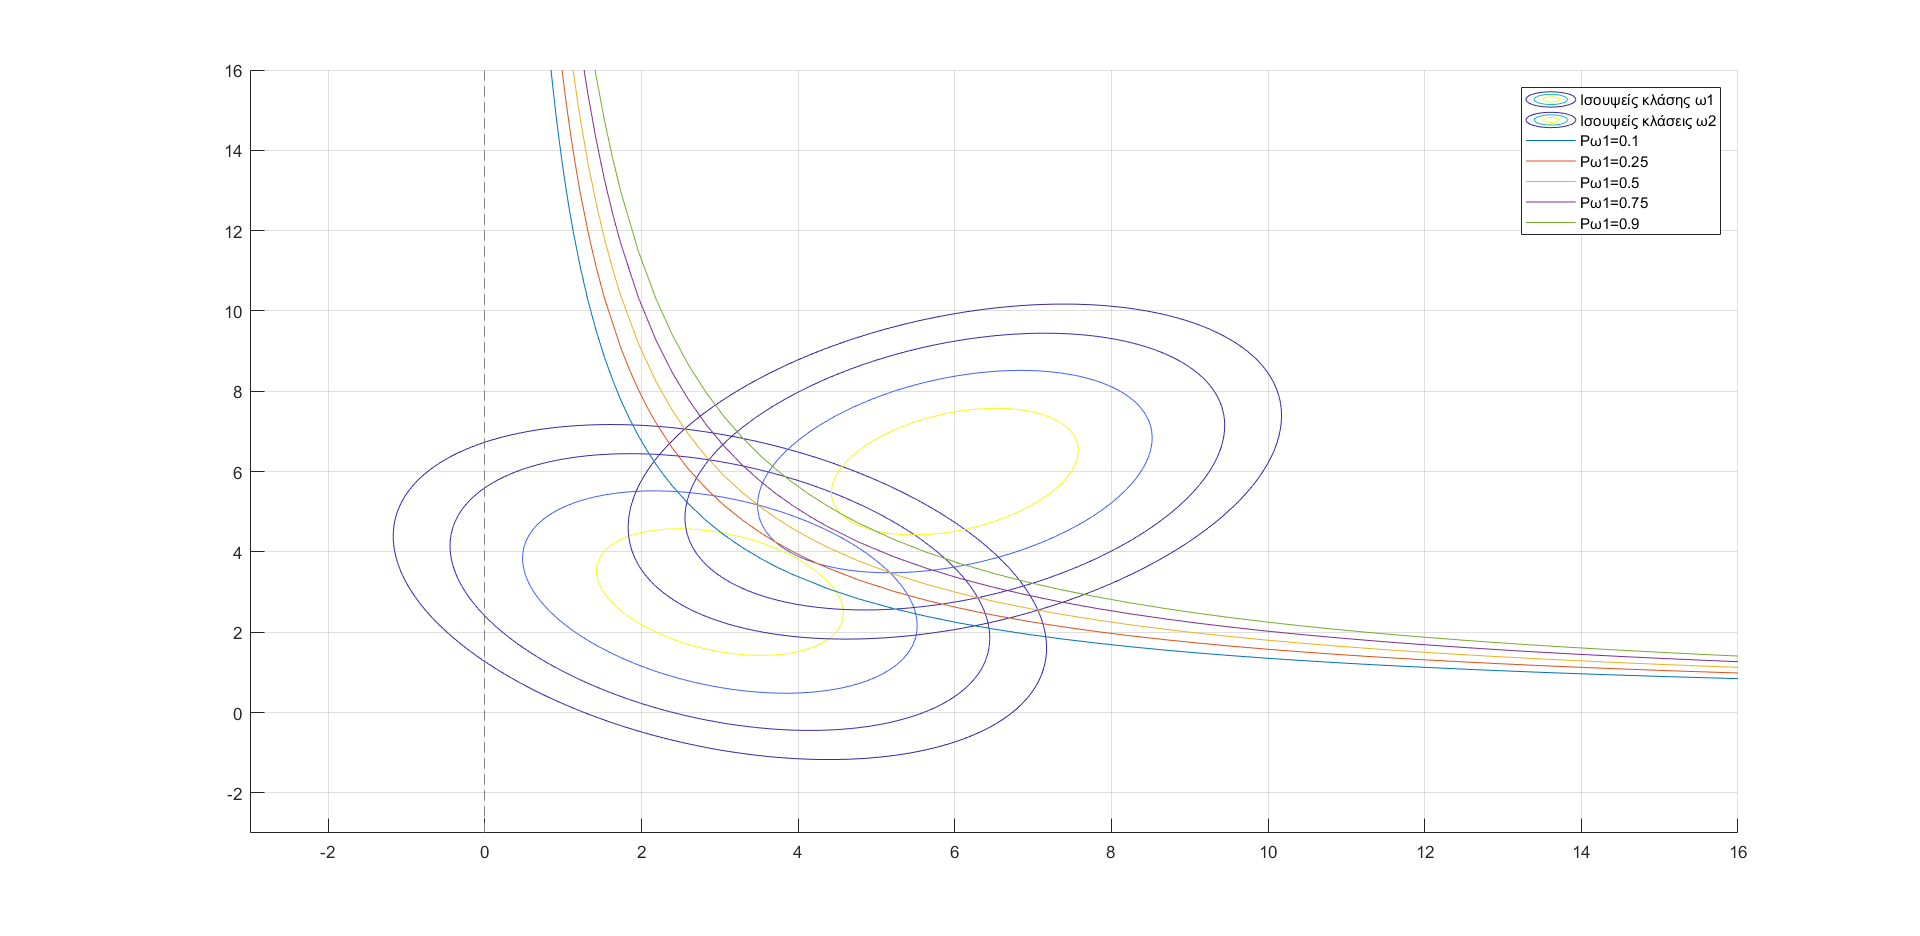
\includegraphics[width=\linewidth]{../exercise1_4/images/part_a.png}
			\caption{Για διαφορετικού πίνακες συνδιασποράς}
		\end{subfigure}%
		~
		\begin{subfigure}[t]{0.5\textwidth}
			\centering
			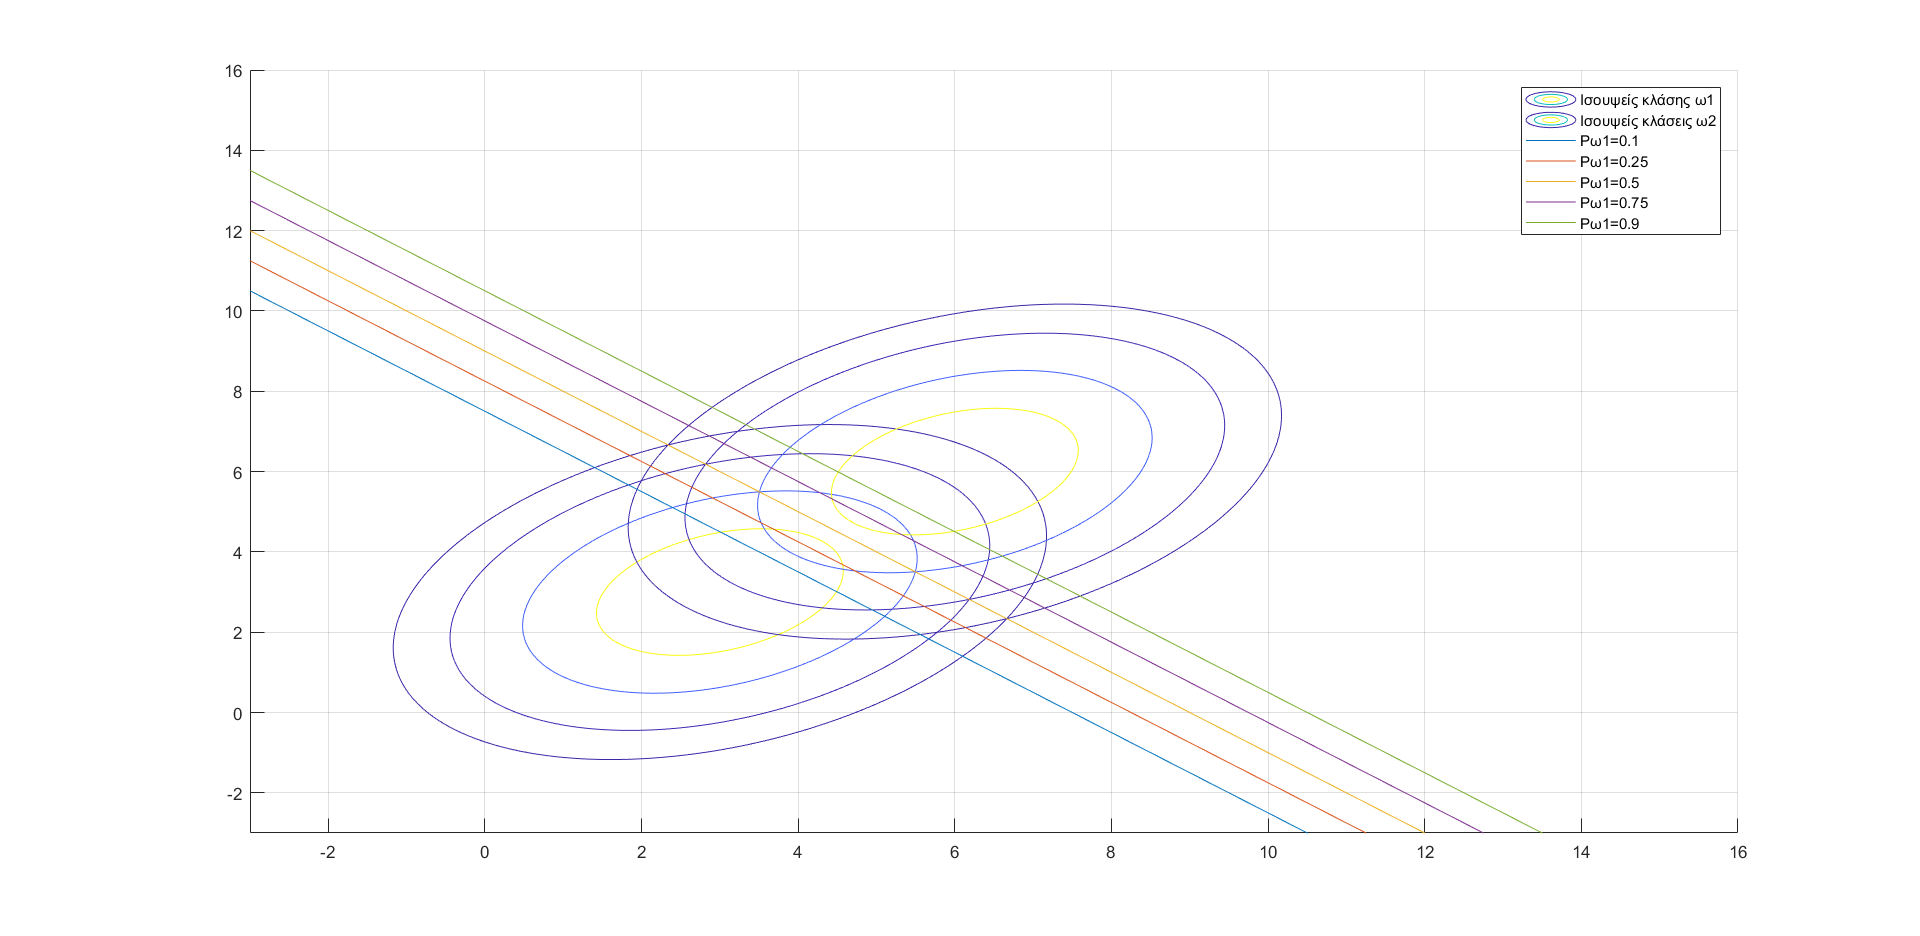
\includegraphics[width=\linewidth]{../exercise1_4/images/part_b.png}
			\caption{Για ίδιους πίνακες συνδιασποράς}
		\end{subfigure}
	\end{figure}

	\noindent
	Από τις παραπάνω εικόνες παρατηρούμε ότι τα σύνορα απόφασης για διαφορετικούς πίνακες συνδιασποράς έχουν τη μορφή υπερβολής και όσο αυξάνεται η πιθανότητα P($ω_{1}$) τόσο μεγαλώνει η περιοχή απόφασης της κλάσης $ω_{1}$ και τα σύνορα απόφασης πλησιάζουν προς το κέντρο της Γκαουσιανής της κλάσης $ω_{2}$. Στην περίπτωση που έχουμε ίδιους πίνακες συνδιασποράς τότε η μορφή του ορίου απόφασης γίνεται γραμμική, ενώ πάλι με την αύξηση της P($ω_{1}$) παρατηρούμε το ίδιο με την περίπτωση όπου είχαμε διαφορετικούς πίνακες συνδιασποράς για τις δύο κλάσεις.
	
	\pagebreak
\section*{Άσκηση 5: Εξαγωγή χαρακτηριστικών και Bayes Classification}
	Σκοπός αυτής της άσκησης είναι να δημιουργήσουμε έναν απλό ταξινομητή Bayes ο οποίος θα ταξινομεί δείγματα σε δύο κλάσεις και συγκεκριμένα στις κλάσεις $C_{1}$ και $C_{2}$ των ψηφίων 1 και 2 αντίστοιχα που βρίσκονται στο αρχείο 'minst.mat'.\\
	
	\noindent
	Αρχικά, δημιουργήθηκε μία συνάρτηση computeAspectRatio() με την οποία υπολογίζουμε το ελάχιστο παραλληλόγραμμο που περικλύει το κάθε ψηφίο που απείκονίζεται στις εικόνες. Ειδικότερα, με αυτό που υπολογίζουμε είναι το height και το width των παραλληλογράμμων και επιστρέφουμε το λόγο $\frac{width}{height}$ της κάθε εικόνας.\\
	
	\noindent
	Στη συνέχεια. υπολογίζουμε για όλες τις εικόνες της κλάσης $C_{1}$ και $C_{2}$ το aspect ratio με τη συνάρτηση που υλοποιήσαμε. Το ελάχιστο aspect ratio βρέθηκε ότι είναι 0.0526, ενώ το μέγιστο 2.375. Eπιπλέον, παρακάτω παρουσιάζονται η εικόνα 50 από την πρώτη κλάση και η εικόνα 500 από τη 2η κλάση μαζί με τα αντίστοιχα παραλληλόγραμμα που περικλύουν τα ψηφία
	
	\begin{figure}[h!]
		\centering
		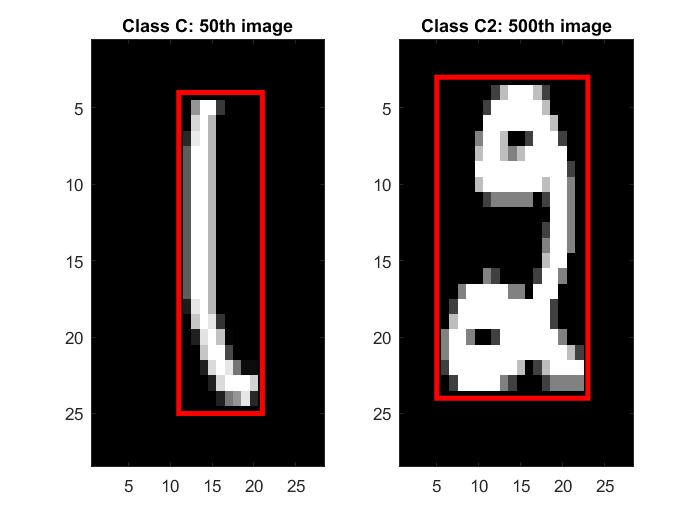
\includegraphics[width=\linewidth]{../exercise1_5/images/c1_c2_digits.png}
	\end{figure}

	\noindent
	Kατόπιν, υπολογίσαμε τις prior πιθανότητες της κάθε κλάσης ως το πηλίκο του αριθμού των εικόνων που έχει η κλάση $C_{i}$ με τον συνολικό αριθμό εικόνων που έχουν οι δύο κλάσεις μαζί. Οι πιθανότητες της κάθε κλάσης αντίστοιχα είναι:

	\begin{itemize}
		\item $P(C_{1}) = 0.5309$ \\ 
		\item $P(C_{2}) = 0.4691$
	\end{itemize}
	
	\pagebreak
	\noindent
	Επιπλέον, η κατανομή του aspect ratio χαρακτηριστικού σε κάθε κλάση ακολουθεί κανονική κατανομή με μέση τιμή και συνδιασπορά 
	
	\begin{align*}
		\bar{μ} &= \frac{1}{N} \sum_{i=1}^{N} x_{i} \\
		σ &= \sqrt{\frac{1}{N} \sum_{i=1}^{N} (x_{i} - \bar{μ})^2}
	\end{align*}	
	
	\noindent
	Για το classification της κάθε εικόνας στα δείγματα test υπολογίζουμε το aspect ratio με τη συνάρτηση computeAspectRatio() και στη συνέχεια υπολογίζουμε τις δύο likelihood πιθανότητες με βάση τον τύπο $p(x| C_{i}) = \frac{1}{\sqrt{2π} σ_{i}}e^{-\frac{1}{2}\frac{(x -\bar{μ_{i}})^{2}}{σ_{i}^{2}}}$. Αφού υπολογίσουμε αυτές τις δύο πιθανότητες, υπολογίζουμε τις πιθανότητες a-post eriori πολλαπλασιάζοντας με τις prior της αντίστοιχης κλάσης και, τέλος, βλέπουμε ποια είναι μεγαλύτερη. Στην περίπτωση που ισχύει ότι $p(x| C_{1}) \cdot P(C1) > p(x| C_{2}) \cdot P(C2)$ αποφασίζουμε ότι το δείγμα x ανήκει στην κλάση $C_{1}$, αλλιώς ανήκει στην $C_{2}$. Aφού επαναλάβουμε αυτή τη διαδικασία και για τα δύο σύνολα εικόνων test, υπολογίζουμε το συνολικό ποσοστό σφάλματος του ταξινομητή μας ως το πηλίκο του αριθμού των λανθασμένων αποφάσεων που πήρε ο ταξινομητής με το συνολικό αριθμό εικόνων που κάναμε classify. Το συνολικό σφάλμα υπολογίστηκε ότι είναι περίπου 10.94\%
	
\section*{Άσκηση 6: Minimum risk}
	Έστω ένα πρόβλημα κατηγοριοποίησης σε δύο κλάσεις $ω_1$ και $ω_2$ όπου οι εκ των προτέρων πιθανότητες είναι ίσες $P(ω_1) = P(ω_2)$. Τα δείγματα x που πρέπει να κατηγοριοποιηθούν είναι	μονοδιάστατα και ακολουθούν κατανομή Rayleigh με συνάρτηση πυκνότητας πιθανότηταςη οποία είναι: 
	
	\begin{equation*}
		p(x | ω_{{i}})=
		\begin{cases}
			\frac{x}{σ_{i}^2} \cdot e^{-\frac{x ^{2}}{2 \cdot σ_{i}^{2}}} & x \ge 0 \\
			0 & x < 0
		\end{cases}
	\end{equation*}

	\noindent
	Επιπλέον, $σ_1 = 1$ και $σ_2 = 2$ ενώ ο πίνακας ρίσκου είναι
	
	\begin{align*}
		L = 
		\begin{bmatrix}
			0 & 0.5 \\
			1 & 0
		\end{bmatrix}	
	\end{align*}
	
	\noindent
	Tότε 
	\begin{align*}
		l_1 &= l_{11} \cdot p(ω_1 | x) + l_{21} \cdot p(ω_2 | x) = 
				0 \cdot p(ω_1 | x) + 1 \cdot p(ω_2 | x) =
				 p(ω_2 | x) \\
		l_2 &= l_{12} \cdot p(ω_1 | x) + l_{22} \cdot p(ω_2 | x) = 
				0.5 \cdot p(ω_1 | x) + 0 \cdot p(ω_2 | x) =
				0.5 \cdot p(ω_1 | x)		
	\end{align*}
	
	\noindent
	Για να βρούμε το όριο απόφασης θα πρέπει να λύσουμε την εξίσωση 
	
	\begin{align*}
		l_1 &= 	l_2 \\
		p(ω_2 | x) &= 0.5 \cdot p(ω_1 | x)	\\	
		p(ω_1 | x) &= 2 \cdot p(ω_2 | x) \\
		\frac{x}{σ_{1}^2} \cdot e^{-\frac{x ^{2}}{2 \cdot σ_{1}^{2}}} &= 2 \cdot \frac{x}{σ_{2}^2} \cdot e^{-\frac{x ^{2}}{2 \cdot σ_{2}^{2}}}\\ 
		\frac{x}{1^2} \cdot e^{-\frac{x ^{2}}{2 \cdot 1^{2}}} &= 2 \cdot \frac{x}{2^2} \cdot e^{-\frac{x ^{2}}{2 \cdot 2^{2}}}
	\end{align*}

	\pagebreak
	\begin{align*}
		e^{-\frac{x ^{2}}{2}} &= \frac{1}{2} \cdot e^{-\frac{x ^{2}}{8}} \\
		2 \cdot e^{-\frac{x ^{2}}{2}} &= e^{-\frac{x ^{2}}{8}} \\
		\ln(2) -\frac{x ^{2}}{2} &= -\frac{x ^{2}}{8} \\
		\frac{3 \cdot x ^{2}}{8} &= \ln(2) \\
		x &= \sqrt{\frac{8 \cdot \ln(2)}{3}} \approx 1.36
	\end{align*}
\section*{Άσκηση 7: Singular Value Decomposition (SVD)}
	Έστώ ο παρακάτω πίνακας
	
	\begin{align*}
		X = 
		\begin{bmatrix}
			1 & 2 \\
			2 & 1 \\
			1 & 3
		\end{bmatrix}	
	\end{align*}

	\noindent
	Tότε ο πίνακας $X^TX$ είναι ο εξής
		\begin{align*}
		\begin{bmatrix}
			1 & 2 & 1 \\
			2 & 1 & 3
		\end{bmatrix}
		\cdot
		\begin{bmatrix}
			1 & 2 \\
			2 & 1 \\
			1 & 3
		\end{bmatrix} &= 
		\begin{bmatrix}
			6 & 7 \\
			7 & 14 
		\end{bmatrix}
	\end{align*}

	\begin{align*}
		\det (X^TX - λ \cdot \mathbb{I}) &=
		\det \left(	
		\begin{bmatrix}
			6 & 7 \\
			7 & 14 
		\end{bmatrix} - 
		\begin{bmatrix}
			λ & 0 \\
			0 & λ 
		\end{bmatrix}
		\right) \\ &=
		\det \left(
		\begin{bmatrix}
			6 - λ & 7 \\
			7 & 14 - λ 
		\end{bmatrix}
		\right) \\ &=
		(6 - λ) \cdot (14 - λ) - 49 \\&=
		λ^2 - 20 \cdot λ + 35
	\end{align*}

	\noindent
	Η διακρίνουσα του διωνύμου είναι $Δ = 20^2 - 4 \cdot 1 \cdot 35 = 260$. Oι λύσεις του παραπάνω δυωνύμου είναι: 
	
	\begin{align*}
		λ_{1,2} &= \frac{-(-20 ) \pm \sqrt{260}}{2 \cdot 1} 
				= \frac{20 \pm 2 \cdot \sqrt{65}}{2 } 
				= 10 \pm \sqrt{65}
	\end{align*}

	\noindent
	Συνεπώς, οι ιδιοτιμές του πίνακα $X^TX$ είναι οι παρακάτω
	\begin{align*}
		λ_{1} = 10 + \sqrt{65} = 18.062
		\tab
		λ_{2} = 10 - \sqrt{65} = 1.938
	\end{align*}

	\noindent
	Για να βρούμε τα ιδιοδιανύσματα θα πρέπει να λύσουμε την εξίσωση $(X^TX - λ \cdot \mathbb{I}) \cdot u_{i} = 0$.
	
	\noindent
	Για $λ = 18.062$ έχουμε

	\begin{align*}
		(X^TX - λ \cdot \mathbb{I}) \cdot u_{1} = 0 \Rightarrow
		\left(	
		\begin{bmatrix}
			6 & 7 \\
			7 & 14 
		\end{bmatrix} - 
		\begin{bmatrix}
			18.062 & 0 \\
			0 & 18.062 
		\end{bmatrix}
		\right) 
		\cdot
		\begin{bmatrix}
			u_{11} \\
			u_{12} 
		\end{bmatrix} = 0 \Rightarrow	
		\begin{bmatrix}
			-12.062 & 7 \\
			7 & -4.062 
		\end{bmatrix} 
		\cdot
		\begin{bmatrix}
			u_{11} \\
			u_{12} 
		\end{bmatrix} = 0 \Rightarrow
	\end{align*}

	\pagebreak
	\begin{align*}	
		\begin{bmatrix}
			-12.062 & 7 \\
			7 & -4.062 
		\end{bmatrix} 
		\cdot
		\begin{bmatrix}
			u_{11} \\
			u_{12} 
		\end{bmatrix} = 0 \Rightarrow
		\begin{cases}
			-12.062 \cdot u_{11} + 7 \cdot u_{12} = 0 \\
			7 \cdot u_{11} - 4.062 \cdot u_{12} = 0
		\end{cases} \Rightarrow
		\begin{cases}
			u_{12} = 1.723 \cdot u_{11} \\
			u_{12} = 1.723 \cdot u_{11}
		\end{cases}
	\end{align*}

	\noindent
	Συνεπώς, τα ιδιοδυανίσματα για $λ = 18.062$ είναι της μορφής 
	\begin{align*}	
		u_{1} = k_{1} \cdot
		\begin{bmatrix}
			1 \\
			1.723 
		\end{bmatrix}
	\end{align*}

	\noindent
	Επιπλέον, για να έχουν μέτρο μονάδα θα πρέπει να ισχύει
	\begin{align*}	
		 k_{1}^2 + (1.723 \cdot k_{1})^2 = 1 \Rightarrow 
		 k_{1}^2 + 2.969 \cdot k_{1}^2 = 1 \Rightarrow 
		 3.969 \cdot k_{1}^2 = 1 \Rightarrow
		 k_{1} = \sqrt{\frac{1}{3.969}} \approx 0.5019
	\end{align*}	

	\noindent
	Άρα, καταλλήγουμε στο ιδιοδιάνυσμα
	
	\begin{align*}	
		u_{1} = 
		k_{1} \cdot
		\begin{bmatrix}
			1 \\
			1.723 
		\end{bmatrix} = 
		0.5019 \cdot
		\begin{bmatrix}
			1 \\
			1.723 
		\end{bmatrix} = 
		\begin{bmatrix}
			0.5019 \\
			0.8648 
		\end{bmatrix}
	\end{align*}

	Για $λ = 1.938$ έχουμε
	
	\begin{align*}
		(X^TX - λ \cdot \mathbb{I}) \cdot u_{2} = 0 \Rightarrow
		\left(	
		\begin{bmatrix}
			6 & 7 \\
			7 & 14 
		\end{bmatrix} - 
		\begin{bmatrix}
			1.938 & 0 \\
			0 & 1.938 
		\end{bmatrix}
		\right) 
		\cdot
		\begin{bmatrix}
			u_{21} \\
			u_{22} 
		\end{bmatrix} = 0 \Rightarrow	
		\begin{bmatrix}
			4.062 & 7 \\
			7 & 12.062
		\end{bmatrix} 
		\cdot
		\begin{bmatrix}
			u_{21} \\
			u_{22} 
		\end{bmatrix} = 0 \Rightarrow
	\end{align*}

	\begin{align*}	
		\begin{bmatrix}
			4.062 & 7 \\
			7 & 12.062
		\end{bmatrix} 
		\cdot
		\begin{bmatrix}
			u_{21} \\
			u_{22} 
		\end{bmatrix} = 0 \Rightarrow
		\begin{cases}
			4.062 \cdot u_{21} + 7 \cdot u_{22} = 0 \\
			7 \cdot u_{21} + 12.062 \cdot u_{22} = 0
		\end{cases} \Rightarrow
		\begin{cases}
			u_{21} = -1.723 \cdot u_{22} \\
			u_{21} = -1.723 \cdot u_{22}
		\end{cases}
	\end{align*}

	\noindent
	Συνεπώς, τα ιδιοδυανίσματα για $λ = 1.938$ είναι της μορφής 
	\begin{align*}	
		u_{2} = k_{2} \cdot
		\begin{bmatrix}
			-1.723 \\
			1 
		\end{bmatrix}
	\end{align*}
	
	\noindent
	Επιπλέον, για να έχουν μέτρο μονάδα θα πρέπει να ισχύει
	\begin{align*}	
		(-1.723 \cdot k_{2})^2 + k_{2}^2 = 1 \Rightarrow 
		2.969 \cdot k_{2}^2 + k_{2}^2 = 1 \Rightarrow 
		3.969 \cdot k_{2}^2 = 1 \Rightarrow
		k_{2} = \sqrt{\frac{1}{3.969}} \approx 0.5019
	\end{align*}	
	
	\noindent
	Άρα, καταλλήγουμε στο ιδιοδιάνυσμα
	
	\begin{align*}	
		u_{2} = 
		k_{2} \cdot
		\begin{bmatrix}
			1 \\
			1.723 
		\end{bmatrix} = 
		0.5019 \cdot
		\begin{bmatrix}
			-1.723 \\
			1
		\end{bmatrix} = 
		\begin{bmatrix}
			-0.8648 \\
			0.5019
		\end{bmatrix}
	\end{align*}

	\noindent
	Για τον υπολογισμό των singular values έχουμε ότι $σ_{i} = \sqrt{λ_{i}}$
	\begin{align*}	
		σ_{1} &= \sqrt{λ_{1}} = \sqrt{18.062} \approx 4.25 \\
		σ_{2} &= \sqrt{λ_{2}} = \sqrt{1.938} \approx 1.392
	\end{align*}

	\pagebreak
	\noindent
	Όσον αφορά τον πίνακα $XX^T$ έχουμε
	\begin{align*}
		\begin{bmatrix}
			1 & 2 \\
			2 & 1 \\
			1 & 3
		\end{bmatrix} 
		\cdot 		
		\begin{bmatrix}
			1 & 2 & 1 \\
			2 & 1 & 3
		\end{bmatrix}
		&= 
		\begin{bmatrix}
			5 & 4 & 7 \\
			4 & 5 & 5 \\
			7 & 5 & 10 
		\end{bmatrix}
	\end{align*}
	
	\begin{align*}
		\det (X^TX - λ \cdot \mathbb{I}) &=
		\det \left(	
		\begin{bmatrix}
			5 & 4 & 7 \\
			4 & 5 & 5 \\
			7 & 5 & 10 
		\end{bmatrix} - 
		\begin{bmatrix}
			λ & 0 & 0 \\
			0 & λ & 0 \\
			0 & 0 & λ
		\end{bmatrix}
		\right) =
		\det \left(
		\begin{bmatrix}
			5-λ & 4 & 7 \\
			4 & 5-λ & 5 \\
			7 & 5 & 10-λ 
		\end{bmatrix}
		\right) \\ &=
		(5 - λ) \cdot 
		\det \left(
		\begin{bmatrix}
			5-λ & 5 \\
			5 & 10-λ 
		\end{bmatrix}
		\right) - 
		4 \cdot 
		\det \left(
		\begin{bmatrix}
			4 & 5 \\
			7 & 10-λ 
		\end{bmatrix}
		\right) + 
		7 \cdot 
		\det \left(
		\begin{bmatrix}
			4 & 5-λ \\
			7 & 5 
		\end{bmatrix}
		\right) \\ &=
		(-λ^3 + 20 \cdot λ^2 - 100 \cdot λ + 125) + (16 \cdot λ -20) + (49 \cdot λ - 105) \\ &=
		-λ^3 + 20 \cdot λ^2 - 35 \cdot λ \\ &=
		-λ \cdot (λ^2 - 20 \cdot λ + 35)
	\end{align*}

	\noindent
	Άρα, βλέπουμε ότι ο πίνακας $XX^T$ έχει τις ίδιες ιδιοτιμές με τον πίνακα $X^TX$ και μία επιπλέον ιδιοτιμή την $λ = 0$.\\
	
	\noindent
	Συνεπώς, οι ιδιοτιμές του πίνακα $XX^T$ είναι οι παρακάτω
	\begin{align*}
		λ_{1} = 18.062
		\tab
		λ_{2} =  1.938
		\tab
		λ_{3} = 0
	\end{align*}

	\noindent
	Για $λ = 18.062$ έχουμε
	
	\begin{align*}
		(X^TX - λ \cdot \mathbb{I}) \cdot v_{1} = 0 \Rightarrow
		\left(	
		\begin{bmatrix}
			5 & 4 & 7 \\
			4 & 5 & 5 \\
			7 & 5 & 10 
		\end{bmatrix} - 
		\begin{bmatrix}
			18.062 & 0 & 0 \\
			0 & 18.062 & 0 \\
			0 & 0 & 18.062
		\end{bmatrix}
		\right) 
		\cdot
		\begin{bmatrix}
			v_{11} \\
		    v_{12} \\
		    v_{13}
		\end{bmatrix} &= 0 \Rightarrow\\	
		\begin{bmatrix}
			-13.062 & 4 & 7 \\
			4 & -13.062 & 5 \\
			7 & 5 & -8.062 
		\end{bmatrix}
		\cdot
		\begin{bmatrix}
			v_{11} \\
			v_{12} \\
			v_{13}
		\end{bmatrix} &= 0 \Rightarrow\\
		\begin{cases}
			-13.062 \cdot v_{11} + 4 \cdot v_{12} + 7 \cdot v_{13} = 0 \\
			4 \cdot v_{11} - 13.062 \cdot v_{12} + 5 \cdot v_{13} = 0 \\
			7 \cdot v_{11} + 5 \cdot v_{12} - 8.062 \cdot v_{13} = 0 
		\end{cases} \Rightarrow 
		\begin{cases}
			v_{11} = 0.306 \cdot v_{12} + 0.536 \cdot v_{13}  \\
			v_{11} = 3.2655 \cdot v_{12} - 1.25 \cdot v_{13} \\
			v_{11} = -0.714 \cdot v_{12} + 1.152 \cdot v_{13} 
		\end{cases}
	\end{align*}
	\\
	\noindent
	Aπό τις δύο πρώτες σχέσεις έχουμε ότι
	\begin{align*}	
		 0.306 \cdot v_{12} + 0.536 \cdot v_{13} &= 3.2655 \cdot v_{12} - 1.25 \cdot v_{13} \Rightarrow \\
		  3.2655 \cdot v_{12} -  0.306 \cdot v_{12} &= 0.536 \cdot v_{13} + 1.25 \cdot v_{13} \Rightarrow \\
		  2.9595 \cdot v_{12} &= 1.786 \cdot v_{13} \Rightarrow \\
		  v_{12} &= 0.6035 \cdot v_{13}
	\end{align*}
	
	\noindent
	Αντικαθιστώντας στην τελευταία σχέση προκύπτει ότι
	\begin{align*}	
		v_{11} &= -0.714 \cdot 0.6035 \cdot v_{13} + 1.152 \cdot v_{13} = 0.721 \cdot v_{13}\\
	\end{align*}

	\pagebreak
	\noindent
	Συνεπώς, τα ιδιοδυανίσματα για $λ = 18.062$ είναι της μορφής 
	\begin{align*}	
		v_{1} = k_{1} \cdot
		\begin{bmatrix}
			0.721 \\
			0.6035 \\
			1 
		\end{bmatrix}
	\end{align*}
	
	\noindent
	Επιπλέον, για να έχουν μέτρο μονάδα θα πρέπει να ισχύει
	\begin{align*}	
		(0.721 \cdot k_{1})^2 + (0.6035 \cdot k_{1})^2 + k_{1}^2 = 1 \Rightarrow 
		1.884 \cdot k_{1}^2 = 1 \Rightarrow
		k_{1} = \sqrt{\frac{1}{1.884}} \approx 0.7285
	\end{align*}	
	
	\noindent
	Άρα, καταλλήγουμε στο ιδιοδιάνυσμα
	
	\begin{align*}	
		v_{1} = k_{1} \cdot
		\begin{bmatrix}
			0.721 \\
			0.6035 \\
			1 
		\end{bmatrix} = 
		0.7285 \cdot
		\begin{bmatrix}
			0.721 \\
			0.6035 \\
			1
		\end{bmatrix} = 
		\begin{bmatrix}
			0.5253 \\
			0.4397 \\
			0.7285
		\end{bmatrix}
	\end{align*}

	\noindent
	Για $λ = 1.938$ έχουμε
	
	\begin{align*}
		(X^TX - λ \cdot \mathbb{I}) \cdot v_{2} = 0 \Rightarrow
		\left(	
		\begin{bmatrix}
			5 & 4 & 7 \\
			4 & 5 & 5 \\
			7 & 5 & 10 
		\end{bmatrix} - 
		\begin{bmatrix}
			1.938 & 0 & 0 \\
			0 & 1.938 & 0 \\
			0 & 0 & 1.938
		\end{bmatrix}
		\right) 
		\cdot
		\begin{bmatrix}
			v_{21} \\
			v_{22} \\
			v_{23}
		\end{bmatrix} &= 0 \Rightarrow\\	
		\begin{bmatrix}
			3.062 & 4 & 7 \\
			4 & 3.062 & 5 \\
			7 & 5 & 8.062 
		\end{bmatrix}
		\cdot
		\begin{bmatrix}
			v_{21} \\
			v_{22} \\
			v_{23}
		\end{bmatrix} &= 0 \Rightarrow\\
		\begin{cases}
			3.062 \cdot v_{21} + 4 \cdot v_{22} + 7 \cdot v_{23} = 0 \\
			4 \cdot v_{21} + 3.062 \cdot v_{22} + 5 \cdot v_{23} = 0 \\
			7 \cdot v_{21} + 5 \cdot v_{22} + 8.062 \cdot v_{23} = 0 
		\end{cases} \Rightarrow 
		\begin{cases}
			v_{21} = -1.306 \cdot v_{22} - 2.286 \cdot v_{23} \\
			v_{21} = -0.765 \cdot v_{22} - 1.25 \cdot v_{23} \\
			v_{21} = -0.714 \cdot v_{22} - 1.152 \cdot v_{23} 
		\end{cases}
	\end{align*}
	\\
	\noindent
	Aπό τις δύο πρώτες σχέσεις έχουμε ότι
	\begin{align*}	
		-1.306 \cdot v_{22} - 2.286 \cdot v_{23} &= -0.765 \cdot v_{22} - 1.25 \cdot v_{23} \Rightarrow \\
		1.306 \cdot v_{22} - 0.765 \cdot v_{22} &= - 2.286 \cdot v_{23} + 1.25 \cdot v_{23} \Rightarrow \\
		0.541 \cdot v_{22} &= -1.036 \cdot v_{23} \Rightarrow \\
		v_{22} &= -1.915 \cdot v_{23}
	\end{align*}
	
	\noindent
	Αντικαθιστώντας στην τελευταία σχέση προκύπτει ότι
	\begin{align*}	
			v_{21} = -0.714 \cdot (-1.915 \cdot v_{23}) - 1.152 \cdot v_{23}  = 0.215 \cdot v_{13}\\
	\end{align*}
	
	\noindent
	Συνεπώς, τα ιδιοδυανίσματα για $λ = 1.938$ είναι της μορφής 
	\begin{align*}	
		v_{2} = k_{2} \cdot
		\begin{bmatrix}
			0.215 \\
			-1.915 \\
			1 
		\end{bmatrix}
	\end{align*}
	
	\noindent
	Επιπλέον, για να έχουν μέτρο μονάδα θα πρέπει να ισχύει
	\begin{align*}	
		(0.215 \cdot k_{2})^2 + (-1.915 \cdot k_{2})^2 + k_{2}^2 = 1 \Rightarrow 
		4.713 \cdot k_{2}^2 = 1 \Rightarrow
		k_{2} = \sqrt{\frac{1}{4.713}} \approx 0.4606
	\end{align*}	
	
	\noindent
	Άρα, καταλλήγουμε στο ιδιοδιάνυσμα
	
	\begin{align*}	
		v_{2} = k_{2} \cdot
		\begin{bmatrix}
			0.215 \\
			-1.915 \\
			1 
		\end{bmatrix} = 
		0.4606 \cdot
		\begin{bmatrix}
			0.215 \\
			-1.915 \\
			1 
		\end{bmatrix} = 
		\begin{bmatrix}
			0.099 \\
			0.8821 \\
			0.4606
		\end{bmatrix}
	\end{align*}

	\noindent
	Aν λάβουμε υπόψη μας μόνο τη μεγαλύτερη ιδιοτιμή $λ = 18.062$, τότε το καλύτερο rank-1 approximation προκύπτει ως εξής
	\begin{align*}	
		\tilde{X} &= σ_{1} \cdot u_1 \cdot v_{1}^T \\
				  &= 4.25 \cdot 
				  	 \begin{bmatrix}
				  	 	0.5019 \\
				  	 	0.8648 
				  	 \end{bmatrix}
				  	 \begin{bmatrix}
						0.5253 & 0.4397 & 0.7285
					 \end{bmatrix} \\
				  &= \begin{bmatrix}
				  		1.12 & 1.93 \\ 
				  		0.93 & 1.616 \\
				  		1.554 & 2.68
				  	 \end{bmatrix} 
	\end{align*} 
\end{document}
